\chapter{Test}
\section{Overview and Plan}
The system is tested using bottom-up integration test. Bottom-up integration test is chosen for the system as the system relies heavily on two slave modules. Thus the correctness of the system relies heavily on the two slave modules. Module inputs and user activities are tested using black-box testing to ensure correctness of the system. The root server module (app.js) will be tested alongside with the website functions and its javascripts as http requests must be sent to the server to test its correctness. The test for root server module and website javascripts will be seperated according to the 4 features of the system, user account manipulations, code editing and saving, code compilation and forum.

\section{MySQL Database Interface Module}
\subsection{Purpose}
The connect\_sql.js is tested in this testcase to ensure the correctness of this slave module that act as an interface to communicate between the server and the database. All child classes inherits and reuses the methods of parent class MySQLDatabase, therefore only the major functions of parent class is tested using methods of child classes

\subsection{Inputs}
\subsubsection{Insert}
Test cases of USER used (USERNAME, EMAIL, PASSWORD, ACC\_TYPE):
\begin{enumerate}
  \item newUser, newUser@localhost.net, 11111111, 0 (valid)
  \item (empty), no@here, (empty), 0 (invalid empty input)
  \item no, no, no, no (wrong ACC\_TYPE type)
\end{enumerate}

\subsubsection{Select When All Conditions Are True}
Test cases of SRC\_CODE used (NAME, USER):
\begin{enumerate}
  \item hello\_world.c, 1 (valid)
  \item (empty), 1 (empty name)
  \item here, ADMIN (wrong USER type)
\end{enumerate}

\subsubsection{Delete When All Conditions Are True}
Test cases of SRC\_CODE used (NAME, USER)
\begin{enumerate}
  \item hello-world.c, 1 (valid)
  \item (empty), 1 (empty NAME)
  \item here, ADMIN (wrong USER type)
\end{enumerate}

\subsubsection{Update}
Test cases of USER used (PASSWORD, ID):
\begin{enumerate}
  \item 88888888, 10 (valid)
  \item (empty), 10 (empty PASSWORD)
  \item hello\_goodbye, newUser (wrong ID type)
  \item 88888888, 0 (invalid ID)
\end{enumerate}

\subsection{Expected Outputs \& Pass/Fail Criteria}
The testcases demonstrates the return of the module when different input is provided, both valid and invalid queries to the MySQL database. The module should handle the exception and provide error message for unaccepted invalid testcases and return a ``fail'' message, and provide result for accepted valid or invalid testcases.
\subsubsection{Insert}
Case 1: (pass)
\verbatiminput{Doc/test/case1-1-1.txt}

Case 2: (pass)
\verbatiminput{Doc/test/case1-1-2.txt}

Case 3: (pass)
\lstinputlisting[breaklines]{Doc/test/case1-1-3.txt}

\subsubsection{Select When All Conditions Are True}
Case 1: (pass)
\lstinputlisting[breaklines]{Doc/test/case1-2-1.txt}

Case 2: (pass)
\verbatiminput{Doc/test/case1-2-2.txt}

Case 3: (pass)
\verbatiminput{Doc/test/case1-2-3.txt}

\subsubsection{Delete When All Conditions Are True}
Case 1: (pass)
\verbatiminput{Doc/test/case1-3-1.txt}

Case 2: (pass)
\verbatiminput{Doc/test/case1-3-2.txt}

Case 3: (pass)
\verbatiminput{Doc/test/case1-3-3.txt}

\subsubsection{Update}
Case 1: (pass)
\verbatiminput{Doc/test/case1-4-1.txt}

Case 2: (pass)
\verbatiminput{Doc/test/case1-4-2.txt}

Case 3: (pass)
\verbatiminput{Doc/test/case1-4-3.txt}

Case 4: (pass)
\verbatiminput{Doc/test/case1-4-4.txt}

\section{Source Code Compilation and Execution Module}
\subsection{Purpose}
The compAndRun.js module contains 2 feature, invoke the computer the compile the C source code on the computer, and execute it if there is no error in compilation.

And the testcases observes the result of the compilation and execution.

\subsection{Inputs}
\begin{enumerate}
  \item tmp\_data/hello\_world.c, 1 (valid)
  \item hello\_world.c, 1 (invalid path)
  \item tmp\_data/tmp.txt, 1 (text file instead of c source code file)
  \item tmp\_data/writer.c, 1 (compilation error)
\end{enumerate}

\subsection{Expected Outputs \& Pass/Fail Criteria}
The testcases are supposed to show the possible error message in the middle and show the compilation and execution result in an object at last.

~

Case 1: (pass)
\lstinputlisting[breaklines]{Doc/test/case2-1-1.txt}

Case 2: (pass)
\lstinputlisting[breaklines]{Doc/test/case2-1-2.txt}

Case 3: (pass)
\lstinputlisting[breaklines]{Doc/test/case2-1-3.txt}

Case 4: (pass)
\lstinputlisting[breaklines]{Doc/test/case2-1-4.txt}

\section{Code Handling Module}
\subsection{Purpose}
The code.js module allows save code and compile and execution of source code. Extension names and file names are not concerned by the server.

The testcases observes the result of valid code names and invalid code names when saving and correct code and incorrect code in compilation. The correctness of code fetching will be tested with code compilation as code compilation uses code fetching for source code.

\subsection{Inputs}
\subsubsection{Save Code}
Testcases used (userid, filename, source code):
\begin{enumerate}
  \item 10, hello.c, \verb|#include <stdio.h>\nint main(void)\n{\nprintf("hello world\n");\nreturn 0;\n}| (valid, new code)
  \item 4, hello.c, \verb|#include <stdio.h>\nint main(void)\n{\nprintf("hello world\n");\nreturn 0;\n}| (invalid userid)
  \item 10, hello.c, \verb|#include <stdio.h>\nint main(void)\n{\nprintf("hello world\n");\nreturn 0;\n}| (valid, update code)
  \item 10, (empty string), \verb|#include <stdio.h>\nint main(void)\n{\nprintf("hello world\n");\nreturn 0;\n}| (invalid name)
\end{enumerate}

\subsubsection{Compile and Run}
Testcases used (code id, stdin):
\begin{enumerate}
  \item 12, \verb|""| (valid)
  \item 5, \verb|"98 56\r\n"| (valid with stdin)
  \item 10, \verb|""| (nonexistent code)
  \item 4, \verb|""| (wrong code)
  \item 5, \verb|""| (valid code with invalid input)
\end{enumerate}

\subsection{Expected Outputs \& Pass/Fail Criteria}

\subsubsection{Save Code}
The testcases allows observation of the behaviour of the methos on valid and invalid inputs.

A number indicates a new file created, success indicates successfully updated, and fail indicates failure.

~

Case 1: (pass)
\lstinputlisting[breaklines]{Doc/test/case3-1-1.txt}

Case 2: (pass)
\lstinputlisting[breaklines]{Doc/test/case3-1-2.txt}

Case 3: (pass)
\lstinputlisting[breaklines]{Doc/test/case3-1-3.txt}

Case 4: (pass)
\lstinputlisting[breaklines]{Doc/test/case3-1-4.txt}

\subsubsection{Compile and Run}
The testcases allows us to observe the behaviour of the fetch method and compile and run methos on valid and invalid inputs.

The return of the function should return an object with compilation result and program output on success, and false on failure.

~

Case 1: (pass)
\lstinputlisting[breaklines]{Doc/test/case3-2-1.txt}

Case 2: (pass)
\lstinputlisting[breaklines]{Doc/test/case3-2-2.txt}

Case 3: (pass)
\lstinputlisting[breaklines]{Doc/test/case3-2-3.txt}

Case 4: (pass)
\lstinputlisting[breaklines]{Doc/test/case3-2-4.txt}

Case 5: (pass, random output with invalid stdin)
\lstinputlisting[breaklines]{Doc/test/case3-2-5.txt}

\section{Forum Module}
\subsection{Purpose}
The forum.js handles forum related requests, including fetch post, post posts and replies, search posts, removing posts by authenticated user and fetching basic data of all valid posts in the forum.

The testcases observes the result of each major feature of the module upon valid and invalid posts, and valid and invalid users.

\subsection{Input}
\subsubsection{Fetch Post}
Used testcases (post ID):
\begin{enumerate}
  \item 1 (valid, post)
  \item 2 (valid, reply)
  \item 3 (nonexistent record)
  \item -1 (invalid ID)
  \item 0 (invalid ID)
\end{enumerate}

\subsubsection{Post Post}
Used testcases (title, content, code ID):
\begin{enumerate}
  \item new entry, \verb|something here\r\nand hello world|, 1 (valid)
  \item My first code, \verb|here|, 1 (title collision of another post by different person)
  \item My first code, \verb|here|, 1 (title collision of another post by same person)
  \item (empty string), (empty string), 1 (empty string)
  \item first code, \verb|here|, 0 (invalid code ID)
  \item My first code, \verb|here|, 1 (invalid user)
\end{enumerate}

\subsubsection{Post Reply}
Used testcases (post ID, content):
\begin{enumerate}
  \item 39, \verb|here\r\nhere| (valid)
  \item 43, \verb|here\r\nhere| (reply pointing to a reply, but not post)
  \item 3, \verb|here\r\nhere| (reply pointing to nonexistent entry)
  \item 39, (empty string) (empty reply)
  \item 1, \verb|here\r\nhere| (invalid user)
\end{enumerate}

\subsubsection{Remove Post}
Used testcases (post ID):
\begin{enumerate}
  \item 39 (valid)
  \item 3 (nonexistent entry)
  \item 38 (entry not owned)
\end{enumerate}

\subsubsection{Search}
User testcases (keyword):
\begin{enumerate}
  \item ADMIN (valid username)
  \item C++ (valid titile keyword)
  \item C++ C (valid multiple title keyword with no occurence)
  \item is (valid content keyword)
  \item \#* (valid keyword with universal sign with no occurence)
  \item C* (valid title keyword with universal sign)
\end{enumerate}

\subsubsection{Title Retrieval}
This function requires no specific input

\subsection{Expected Outputs \& Pass/Fail Criteria}
\subsubsection{Fetch Post}
The method should return post with details (author, content, title, code) and all its replies with its author and content

~

Case 1: (pass)
\lstinputlisting[breaklines]{Doc/test/case4-1-1.txt}

Case 2: (pass)
\lstinputlisting[breaklines]{Doc/test/case4-1-2.txt}

Case 3: (pass)
\lstinputlisting[breaklines]{Doc/test/case4-1-3.txt}

Case 4: (pass)
\lstinputlisting[breaklines]{Doc/test/case4-1-4.txt}

Case 5: (pass)
\lstinputlisting[breaklines]{Doc/test/case4-1-5.txt}

For case 5, although the behaviour of it was unexpected, and returns all post heads, but it follows the return format required, therefore it is considered to have the test passed

\subsubsection{Post Post}
The method should return post id upon success.

~

Case 1: (pass)
\lstinputlisting[breaklines]{Doc/test/case4-2-1.txt}

Case 2: (pass)
\lstinputlisting[breaklines]{Doc/test/case4-2-2.txt}

Case 3: (pass)
\lstinputlisting[breaklines]{Doc/test/case4-2-3.txt}

Case 4: (pass)
\lstinputlisting[breaklines]{Doc/test/case4-2-4.txt}

Case 5: (pass)
\lstinputlisting[breaklines]{Doc/test/case4-2-5.txt}

Case 6: (pass)
\lstinputlisting[breaklines]{Doc/test/case4-2-6.txt}

\subsubsection{Post Reply}
The method should return post id of the reply upon success

~

Case 1: (pass)
\lstinputlisting[breaklines]{Doc/test/case4-3-1.txt}

Case 2: (fail)
\lstinputlisting[breaklines]{Doc/test/case4-3-2.txt}

Case 3: (fail)
\lstinputlisting[breaklines]{Doc/test/case4-3-3.txt}

Case 4: (pass)
\lstinputlisting[breaklines]{Doc/test/case4-3-4.txt}

Case 5: (pass)
\lstinputlisting[breaklines]{Doc/test/case4-3-5.txt}

~

Although testcase 2, 3 failed, but that should not be considered as a bug as it will not affect the user. It should be considered as a feature which let users to leave invisible posts.

\subsubsection{Remove Post}
The method should return success or fail to indicate the result of action.

~

Case 1: (pass)
\lstinputlisting[breaklines]{Doc/test/case4-4-1.txt}

Case 2: (pass)
\lstinputlisting[breaklines]{Doc/test/case4-4-2.txt}

Case 3: (pass)
\lstinputlisting[breaklines]{Doc/test/case4-4-3.txt}

\subsubsection{Search}
The method should return related title, author and post id of related posts upon success.

~

Case 1: (pass)
\lstinputlisting[breaklines]{Doc/test/case4-5-1.txt}

Case 2: (pass)
\lstinputlisting[breaklines]{Doc/test/case4-5-2.txt}

Case 3: (pass)
\lstinputlisting[breaklines]{Doc/test/case4-5-3.txt}

Case 4: (pass)
\lstinputlisting[breaklines]{Doc/test/case4-5-4.txt}

Case 5: (pass)
\lstinputlisting[breaklines]{Doc/test/case4-5-5.txt}

Case 6: (pass)
\lstinputlisting[breaklines]{Doc/test/case4-5-6.txt}

\subsubsection{Title Retrieval}
The method should return title, post id, author and created time of all posts, not replies upon success.

~

Case 1: (pass)
\lstinputlisting[breaklines]{Doc/test/case4-6-1.txt}

\section{User Data Handling Module}
Because the module acts as an interface which spawns process of connect\_sql.js MySQL database connection interface module. Therefore the testing of this intermediate module is merged into tests of root server module as decisions are done in root server module and webpage javascripts.

\section{User Account Feature}
\subsection{Purpose}
The system provides user account registration, authentication and personal data retrieval functions to users. Account registration will be tested separately to check whether there is any unwanted behaviour such as allowing blank username or password or repetition of username or user email. User authentication will be checked with user data retrieval as the two functions are closly related.

\subsection{Inputs}
\subsubsection{User Account Registration}
Used testcases (username, email, password, password):
\begin{enumerate}
  \item Joker, joker@dc.com, heath-ledger, heath-ledger (valid)
  \item TEST, test@notest.com, 12345678, 12345678 (used username)
  \item ITEM, test@test.com, 12345678, 12345678 (used email)
  \item hi, hi, 12345678, 12345678 (invalid email address)
  \item hihi, hihi@hihi.net, qwer, qwer (\(\text{password length}<8\))
  \item (empty), incognito@test.com, 12345678, 12345678 (empty username)
  \item hihihi, (empty), 12345678, 12345678 (empty email)
  \item @\#\$xyz, linus@god.com, 12345678, 12345678 (invalid username)
  \item hi, hi@hi.net, 12345678, 456789123 (incorrect re-type of password)
\end{enumerate}

\subsubsection{User Account Authentication and User Data Retrieval}
Used testcase:
\begin{enumerate}
  \item ADMIN, CSCI3100GRP18 (valid normal account)
  \item Joker, 12345678 (wrong password)
  \item AD, CSCI3100GRP18 (invalid username/email)
  \item test@test.com, ABC (valid teacher account using email login)
  \item abc, 11111111 (valid student account)
  \item Joker, Heath-Ledger (different case)
  \item `` or ''``='', a OR 1=1 (SQL injection)
  \item *c*, * (SQL injection)
  \item idk, ``;SELECT * FROM USER WHERE USERNAME=''ADMIN (SQL injection)
\end{enumerate}

\subsection{Expected Outputs \& Pass/Fail Criteria}
\subsubsection{User Account Registration}

Case 1 (pass):

Entered Information with no warning\\
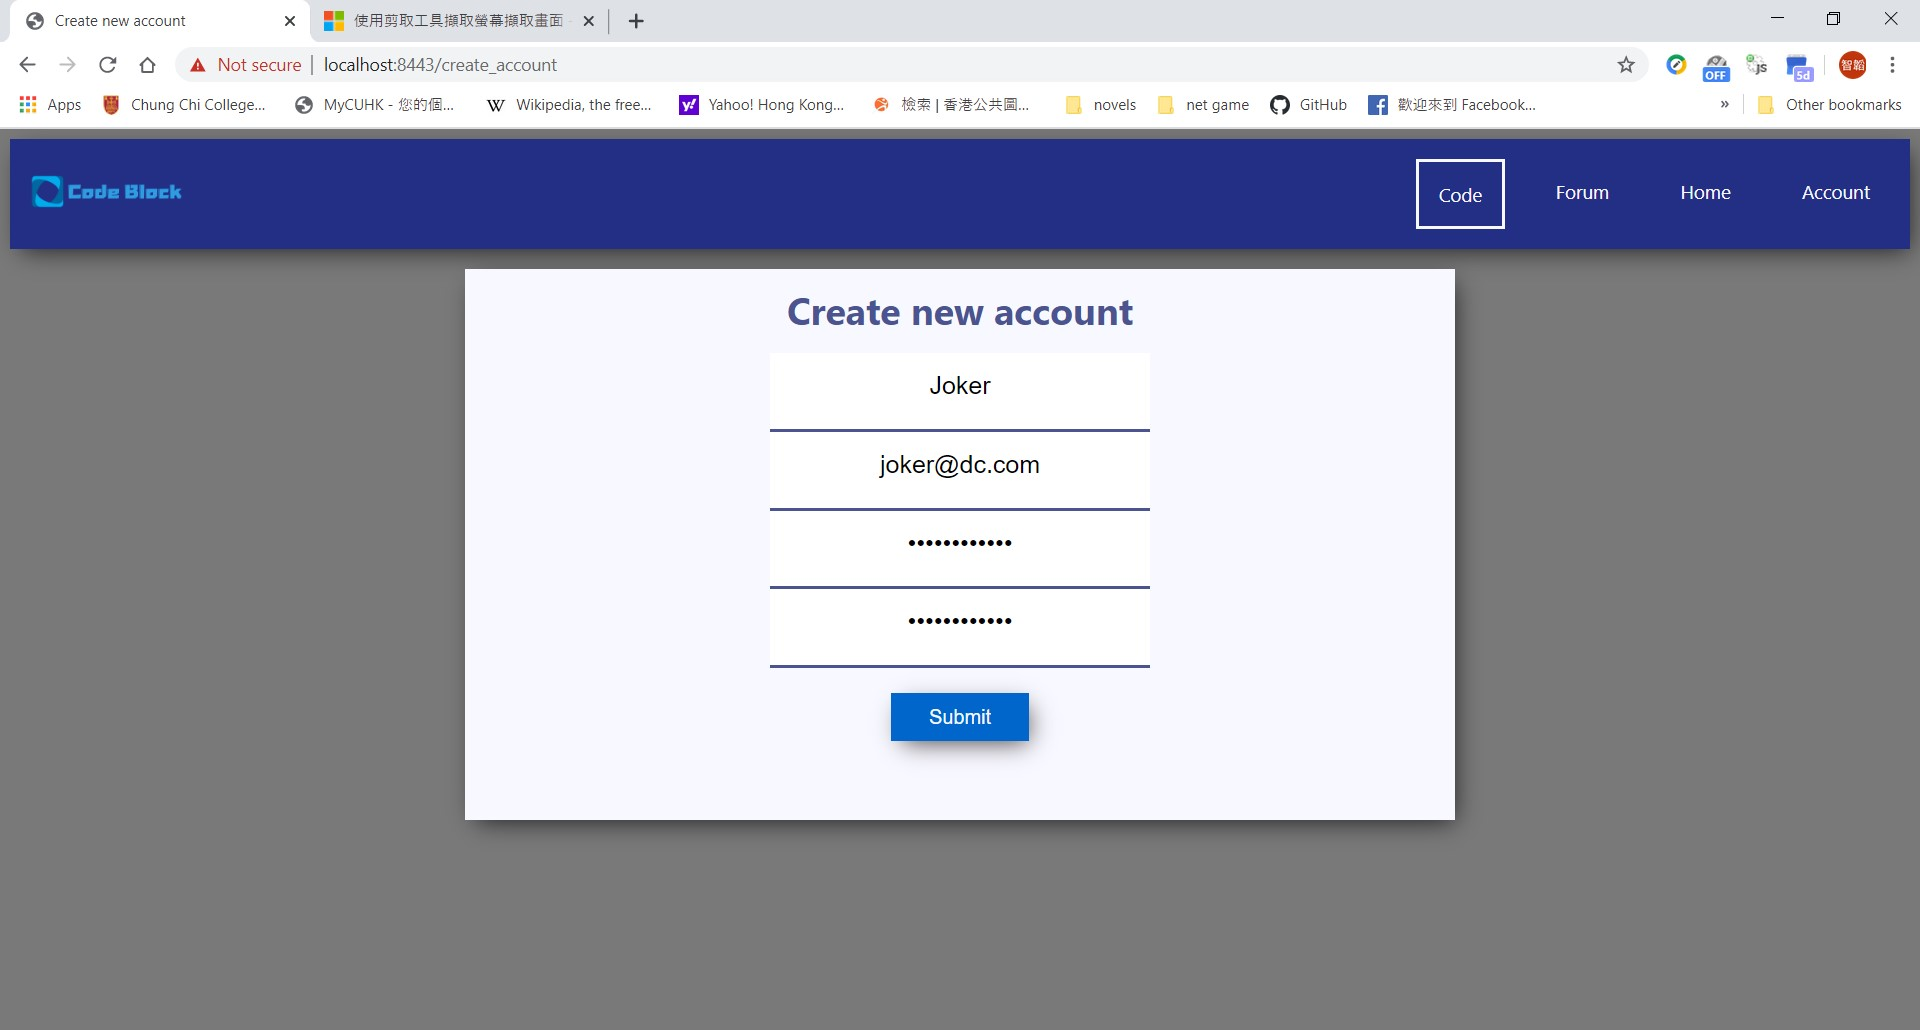
\includegraphics[scale=0.45]{Doc/Pics/case-5-1-1}

Result in shown in terminal\\
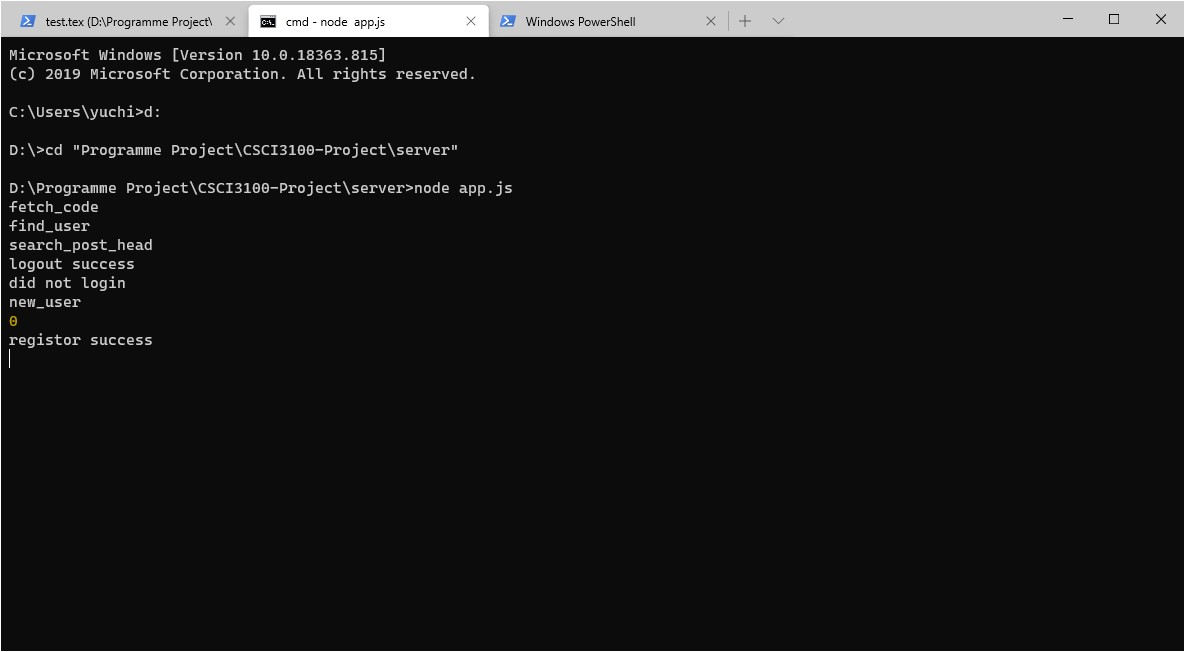
\includegraphics[scale=0.7]{Doc/Pics/case-5-1-1(2)}

User Page\\
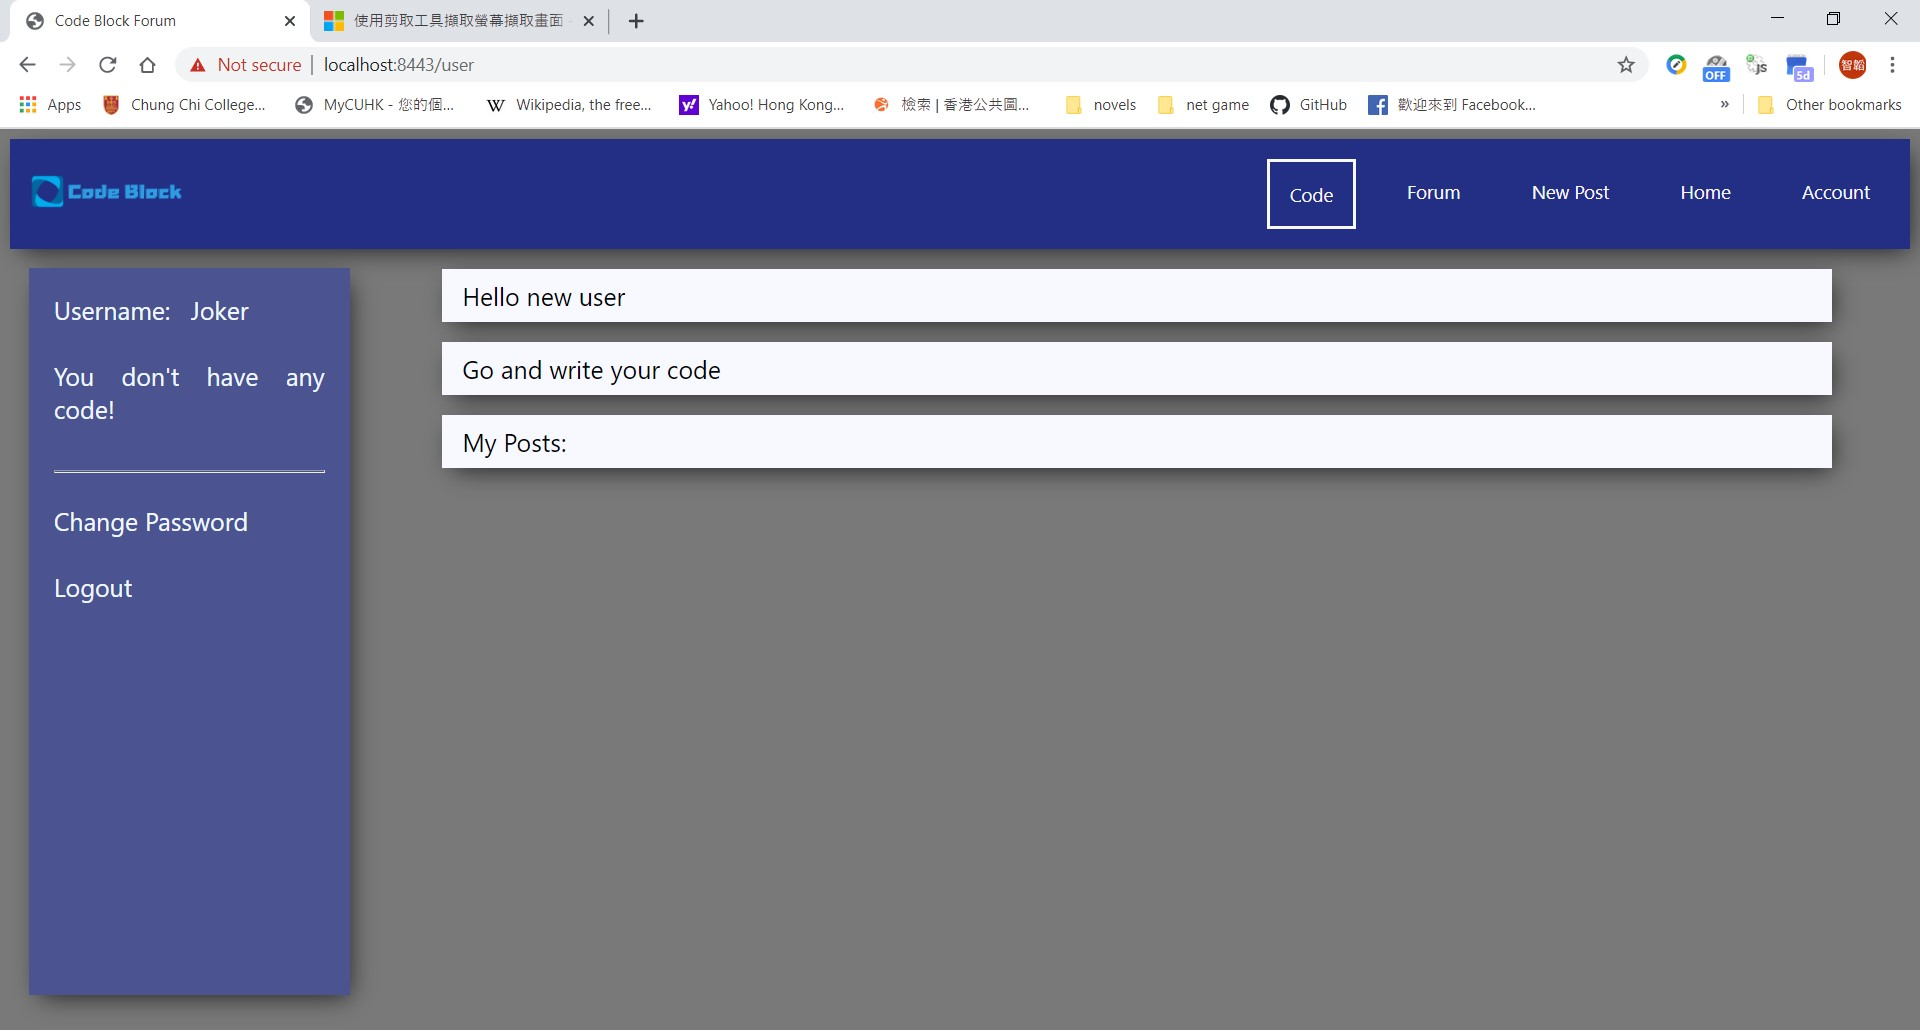
\includegraphics[scale=0.45]{Doc/Pics/case-5-1-1(3)}

~

Case 2: (pass)\\
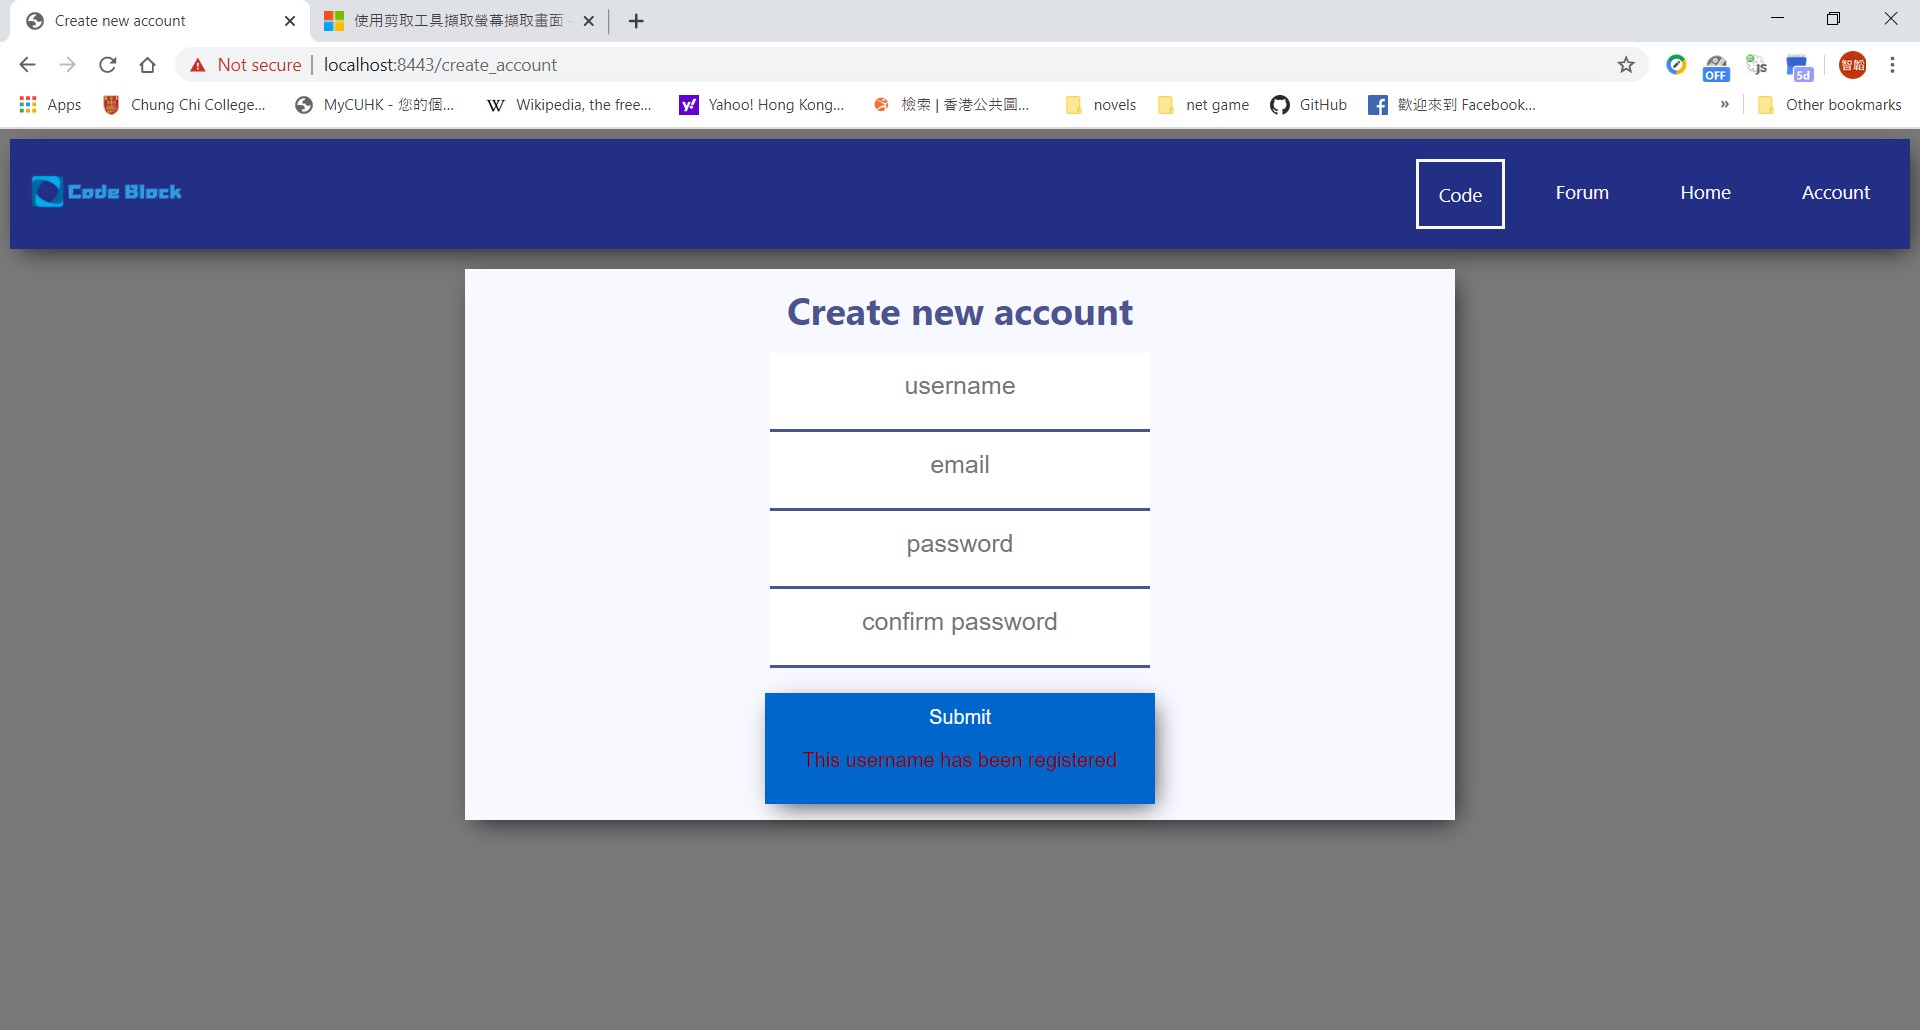
\includegraphics[scale=0.45]{Doc/Pics/case-5-1-2}

~

Case 3: (pass)\\
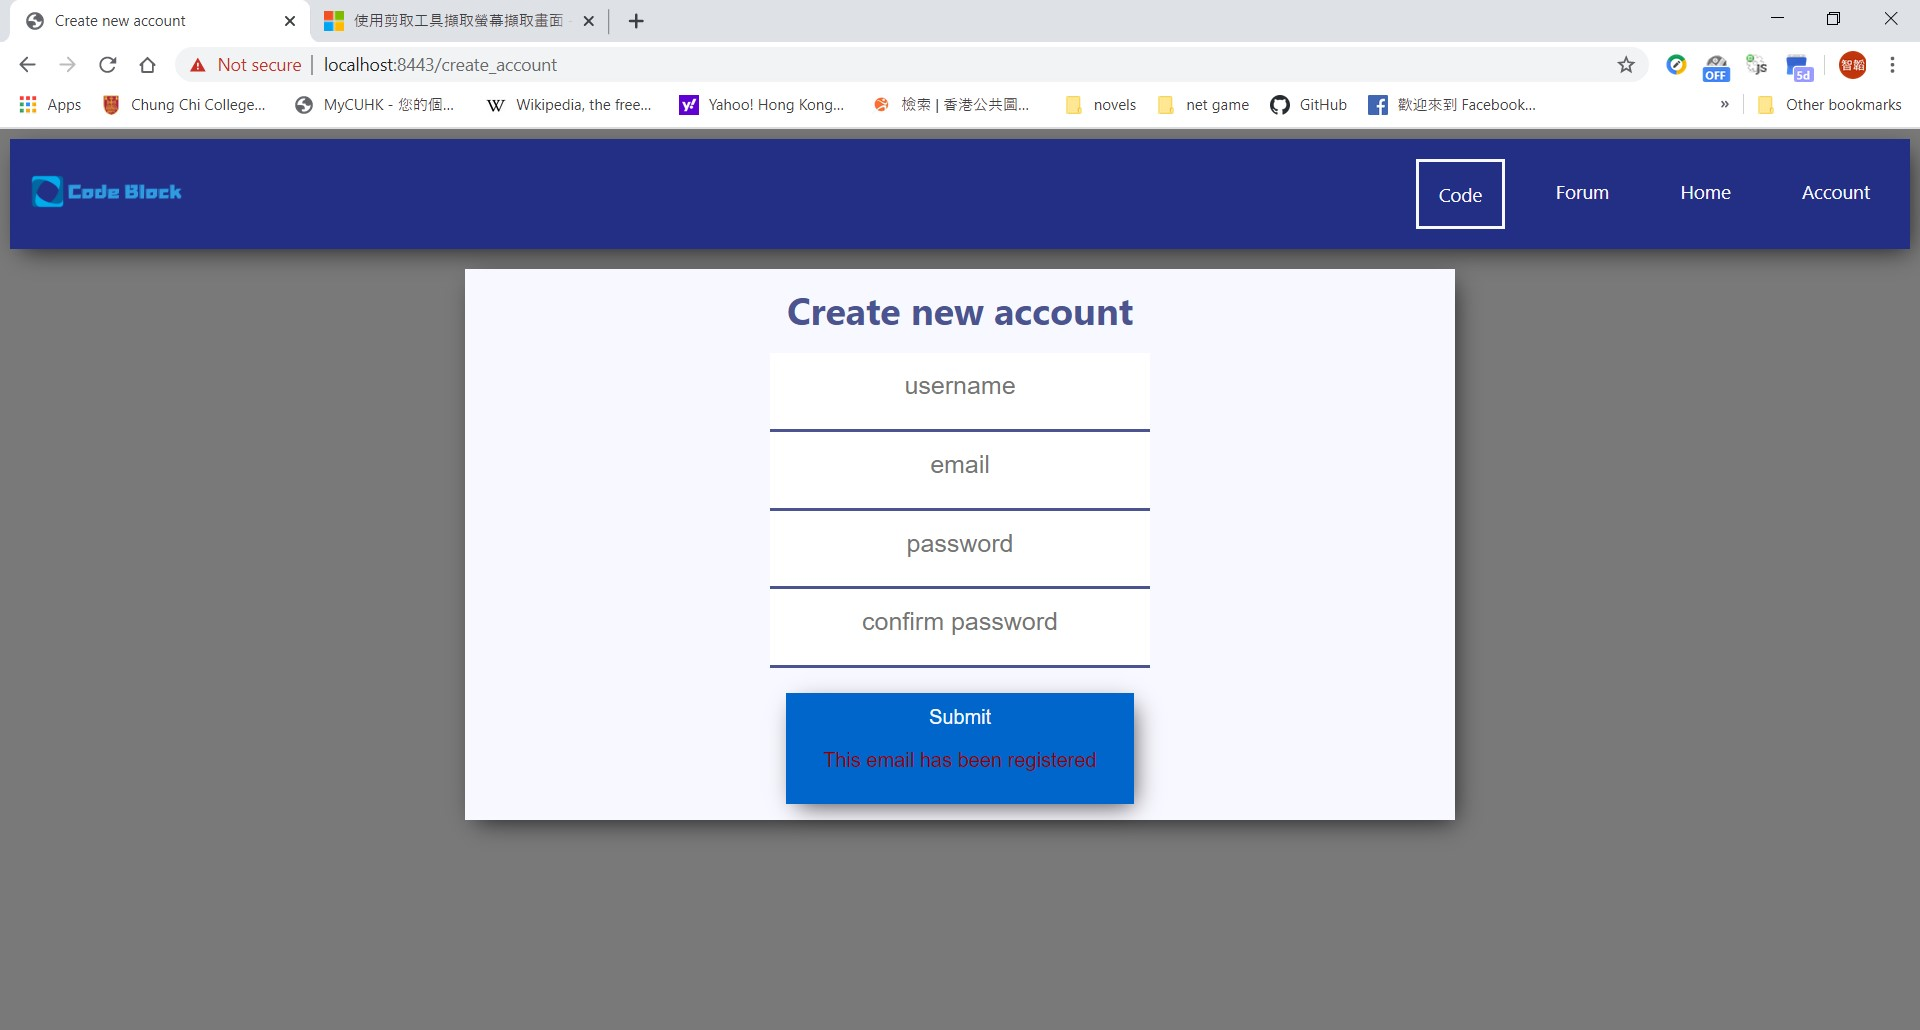
\includegraphics[scale=0.45]{Doc/Pics/case-5-1-3}

~

Case 4: (pass)\\
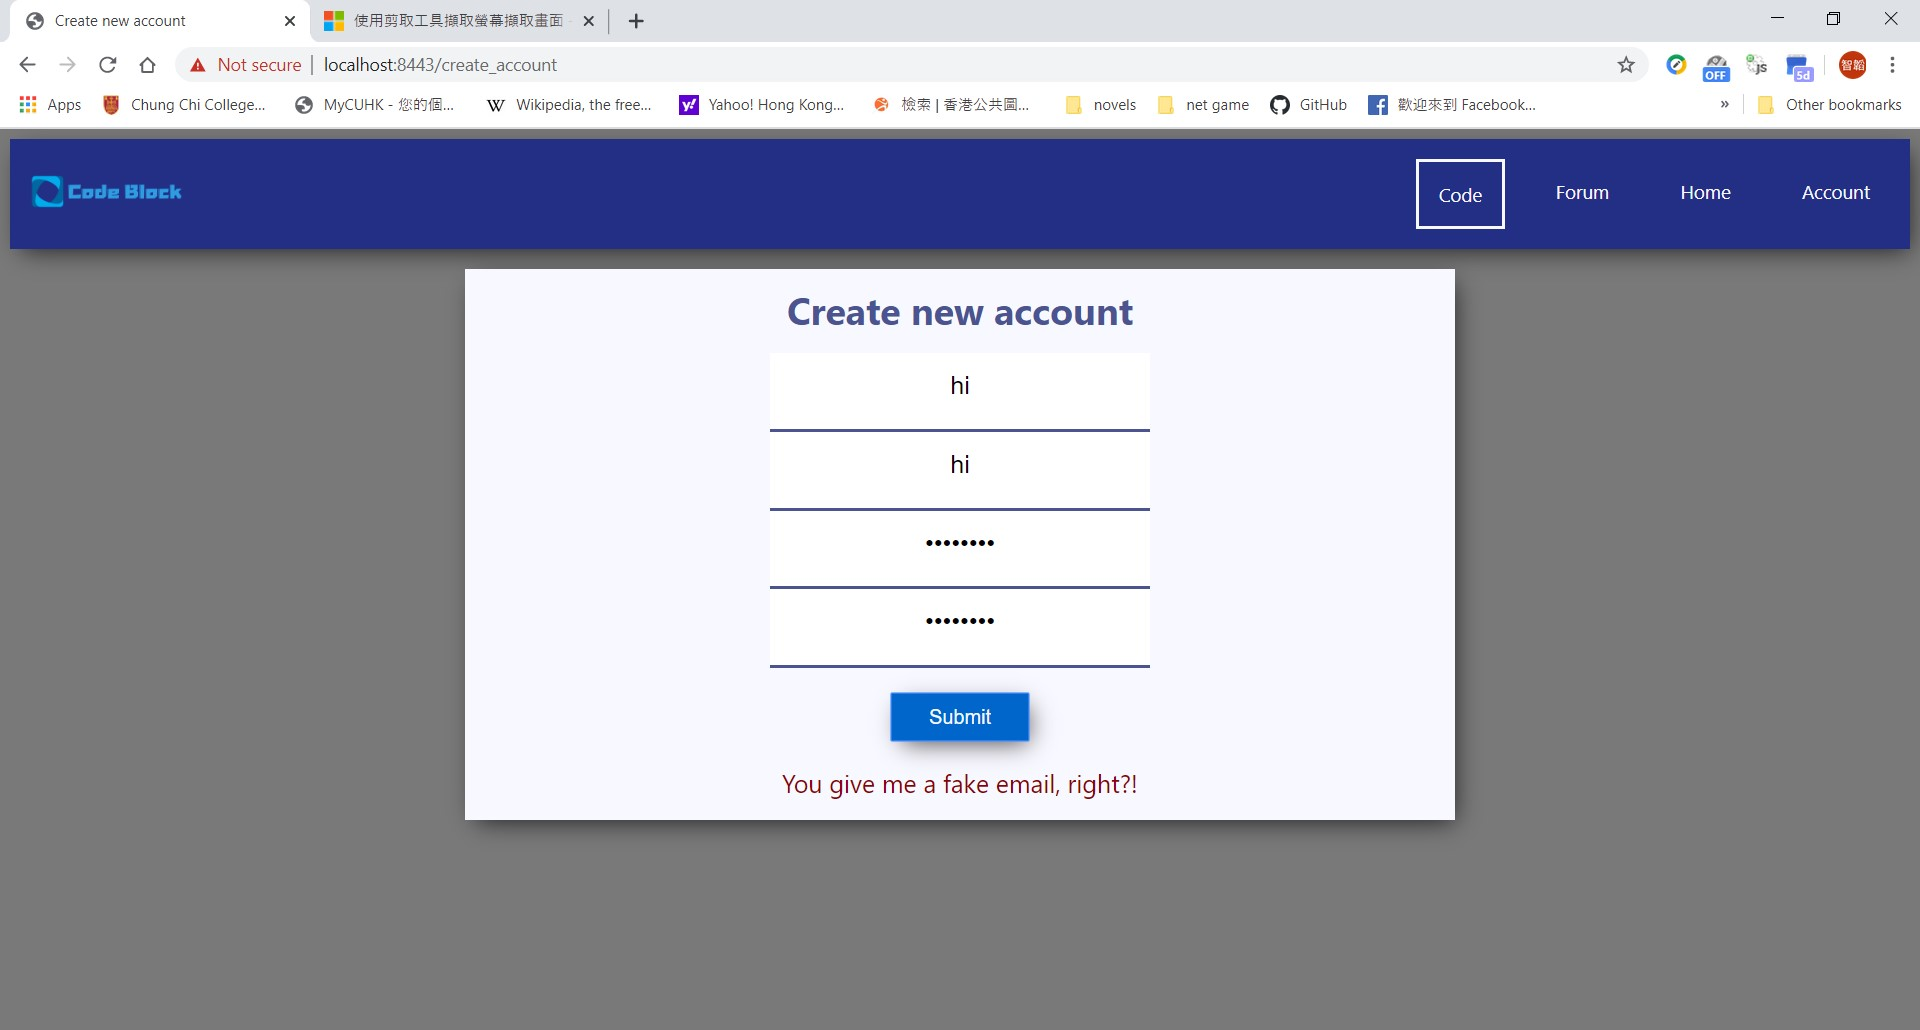
\includegraphics[scale=0.45]{Doc/Pics/case-5-1-4}

~

Case 5: (pass)\\
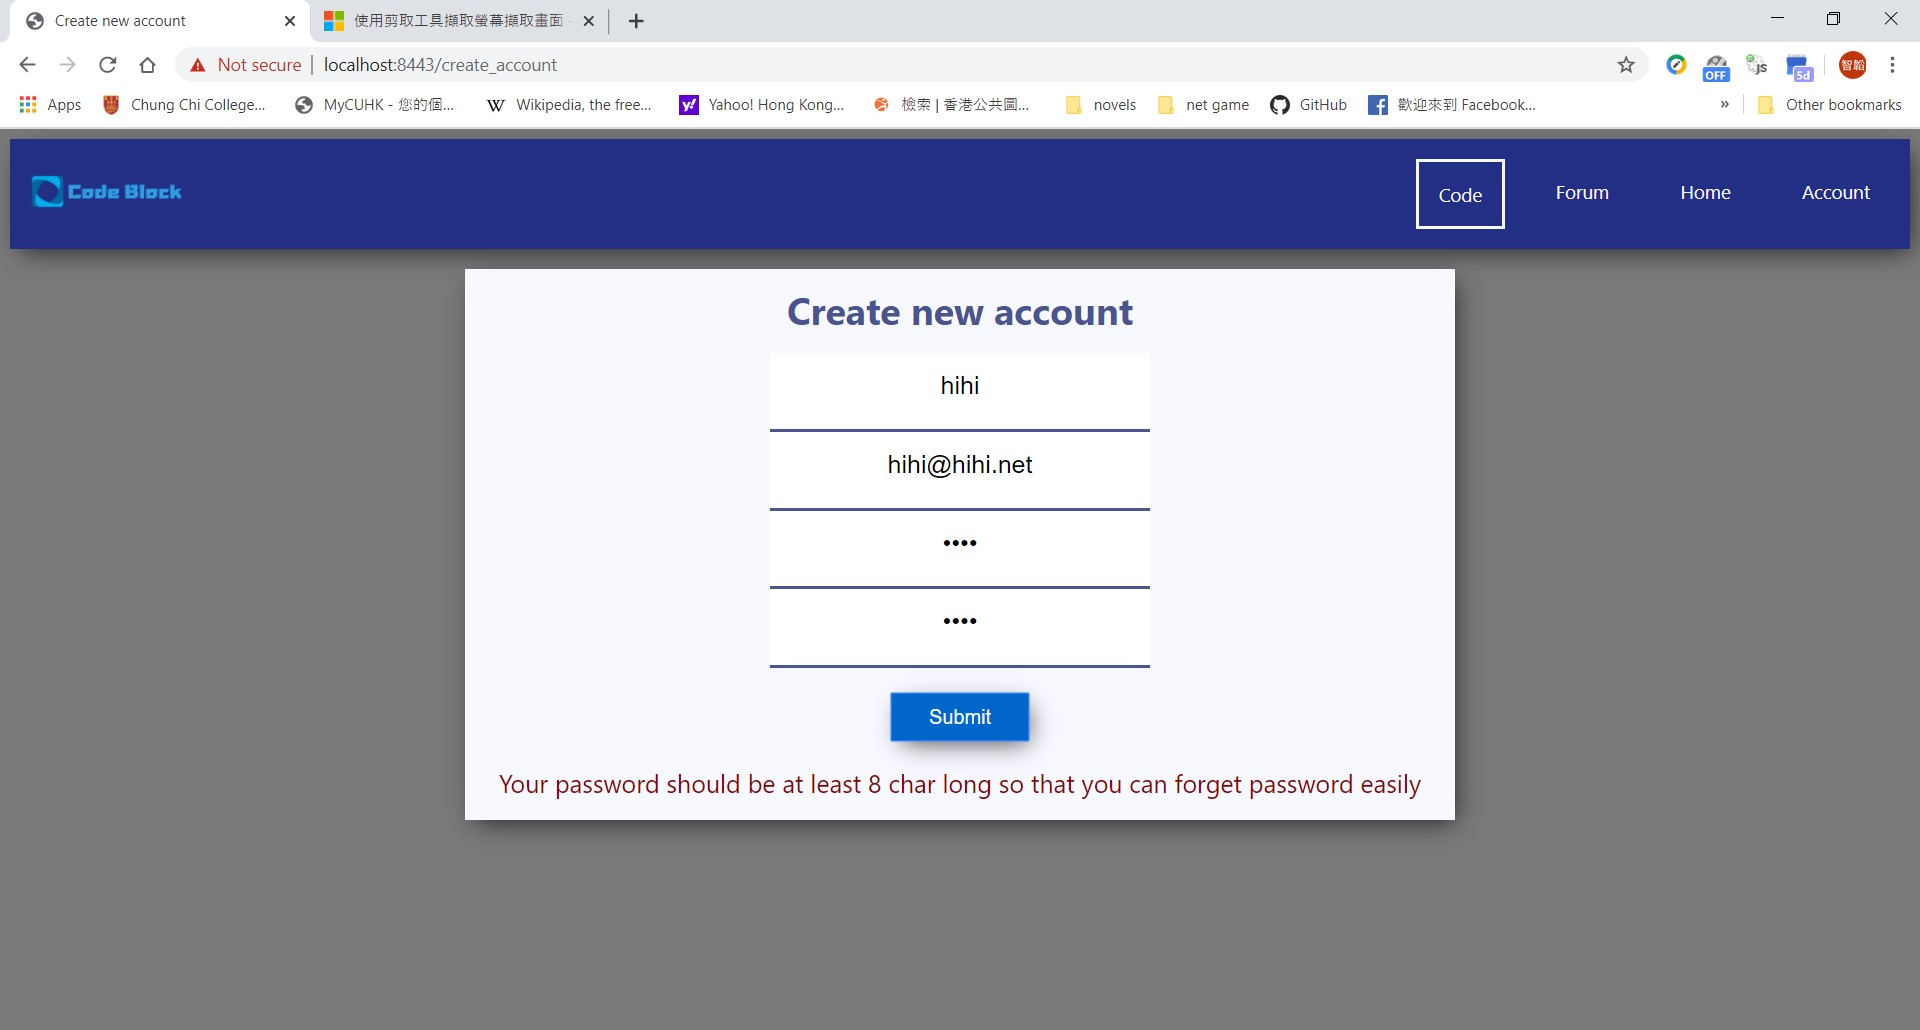
\includegraphics[scale=0.45]{Doc/Pics/case-5-1-5}

~

Case 6: (pass)\\
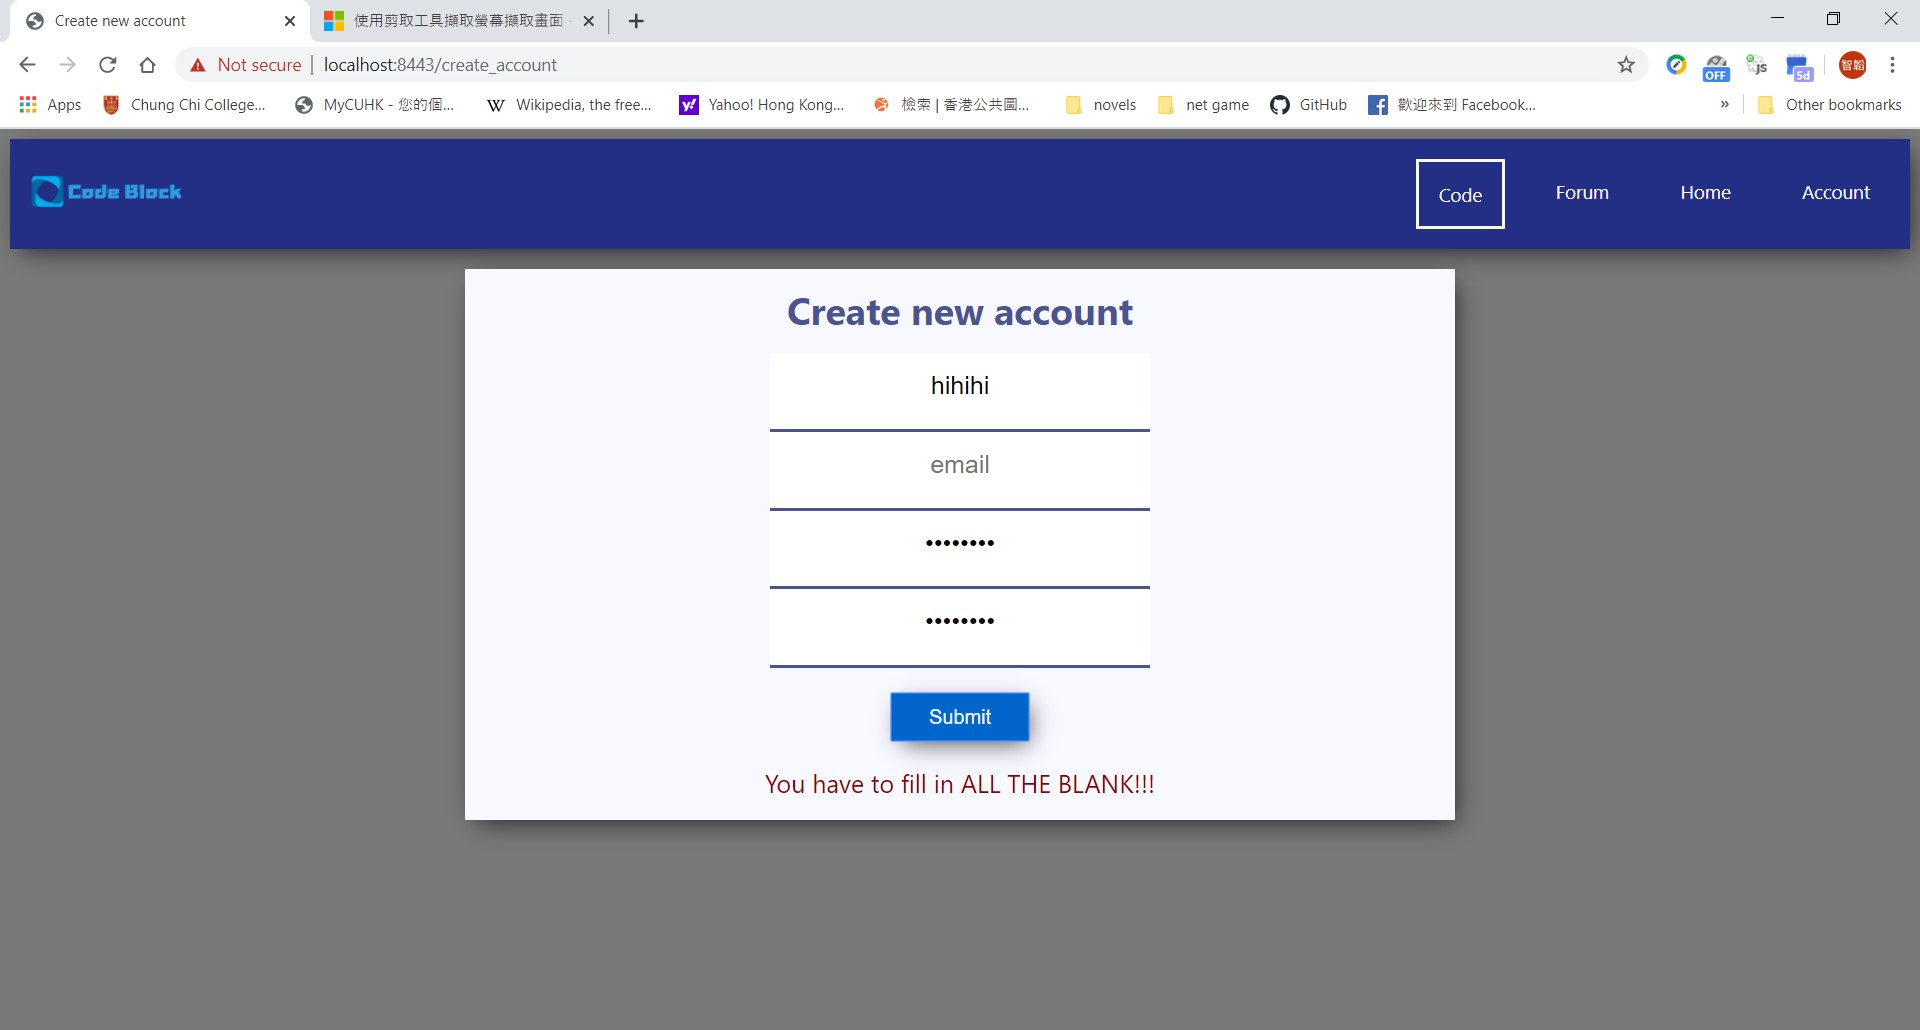
\includegraphics[scale=0.45]{Doc/Pics/case-5-1-6}

~

Case 7: (pass)\\
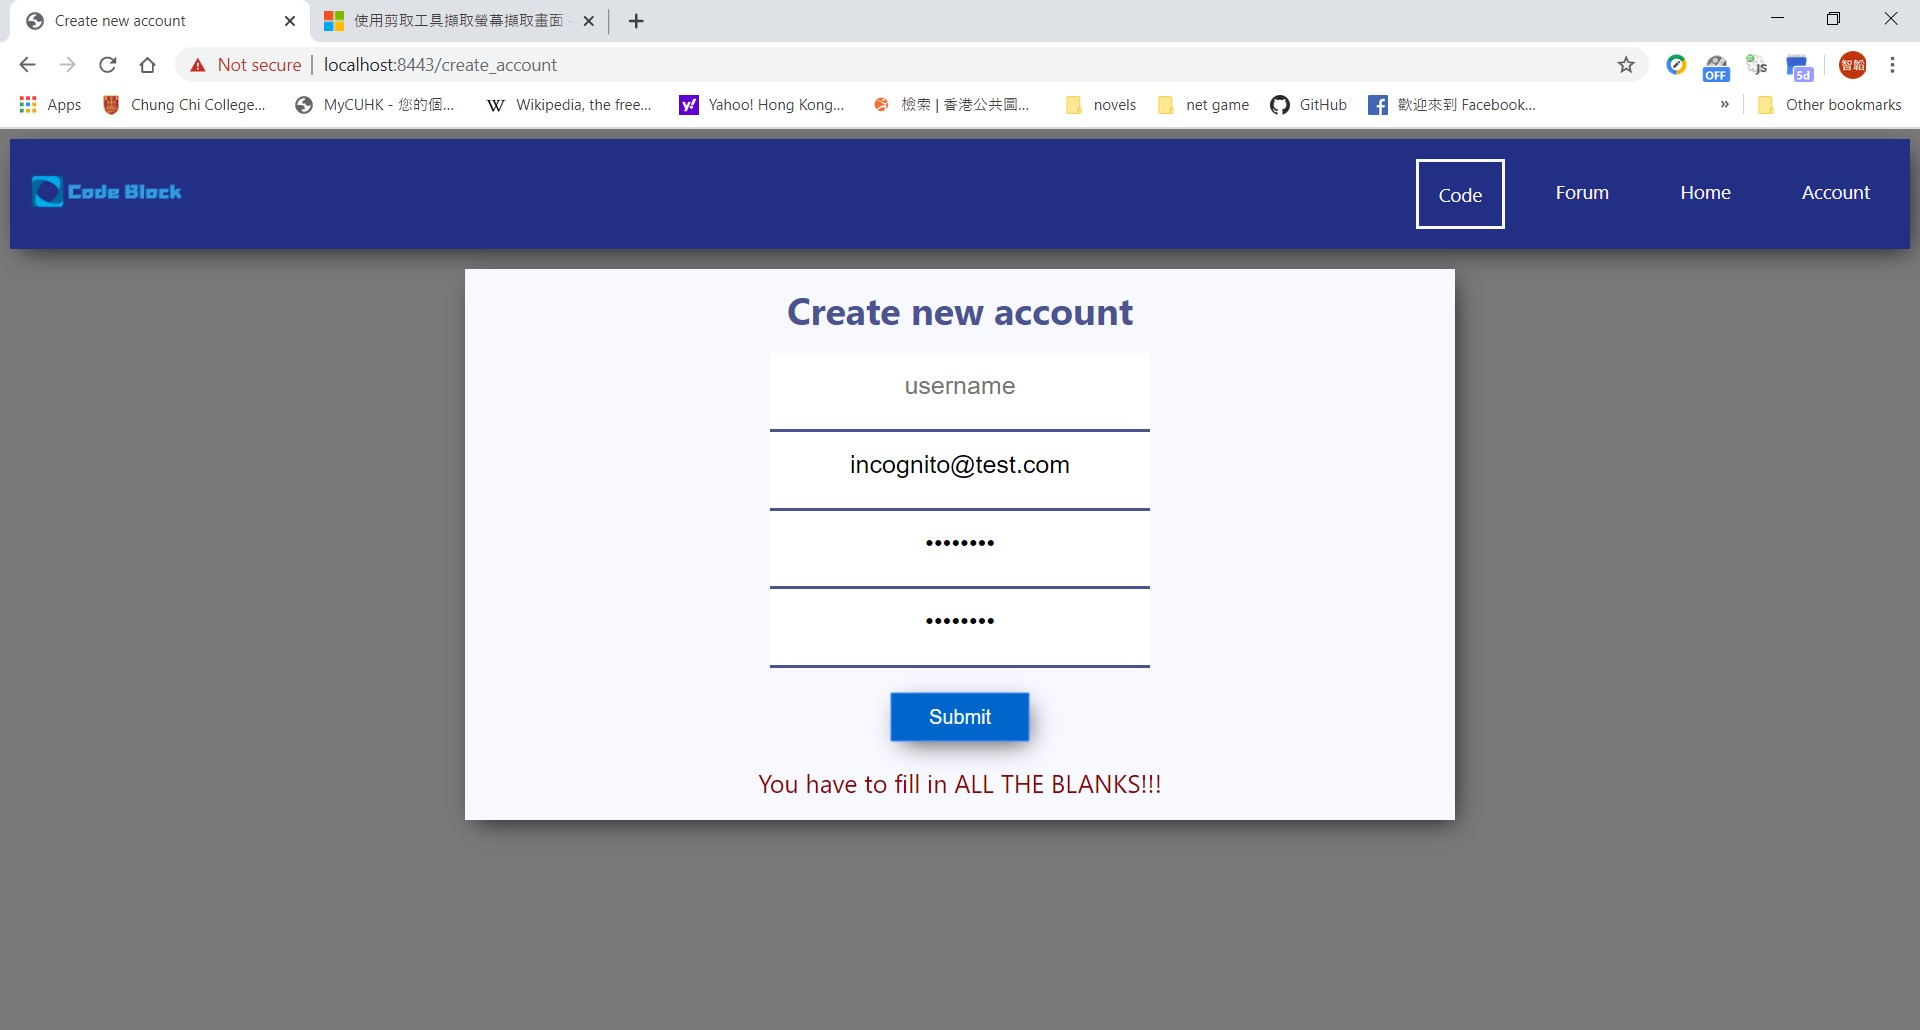
\includegraphics[scale=0.45]{Doc/Pics/case-5-1-7}

~

Case 8: (pass)\\
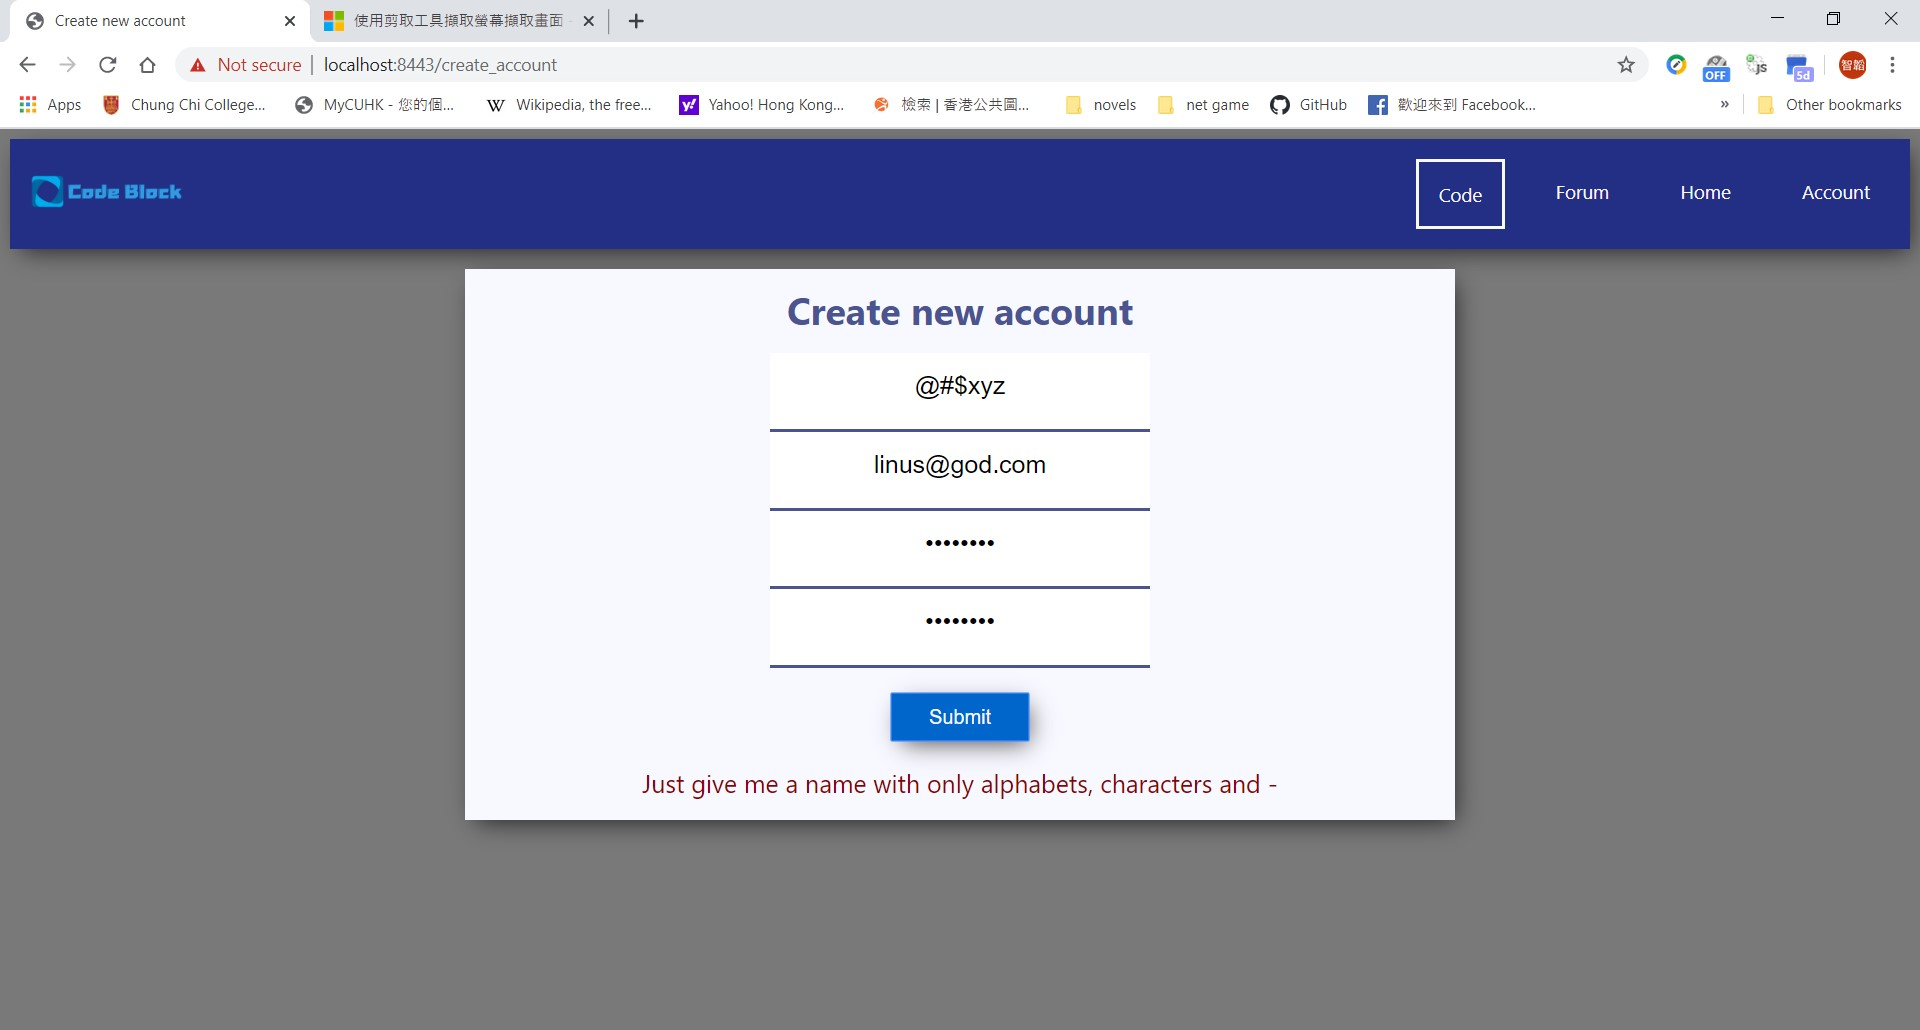
\includegraphics[scale=0.45]{Doc/Pics/case-5-1-8}

~

Case 9: (pass)\\
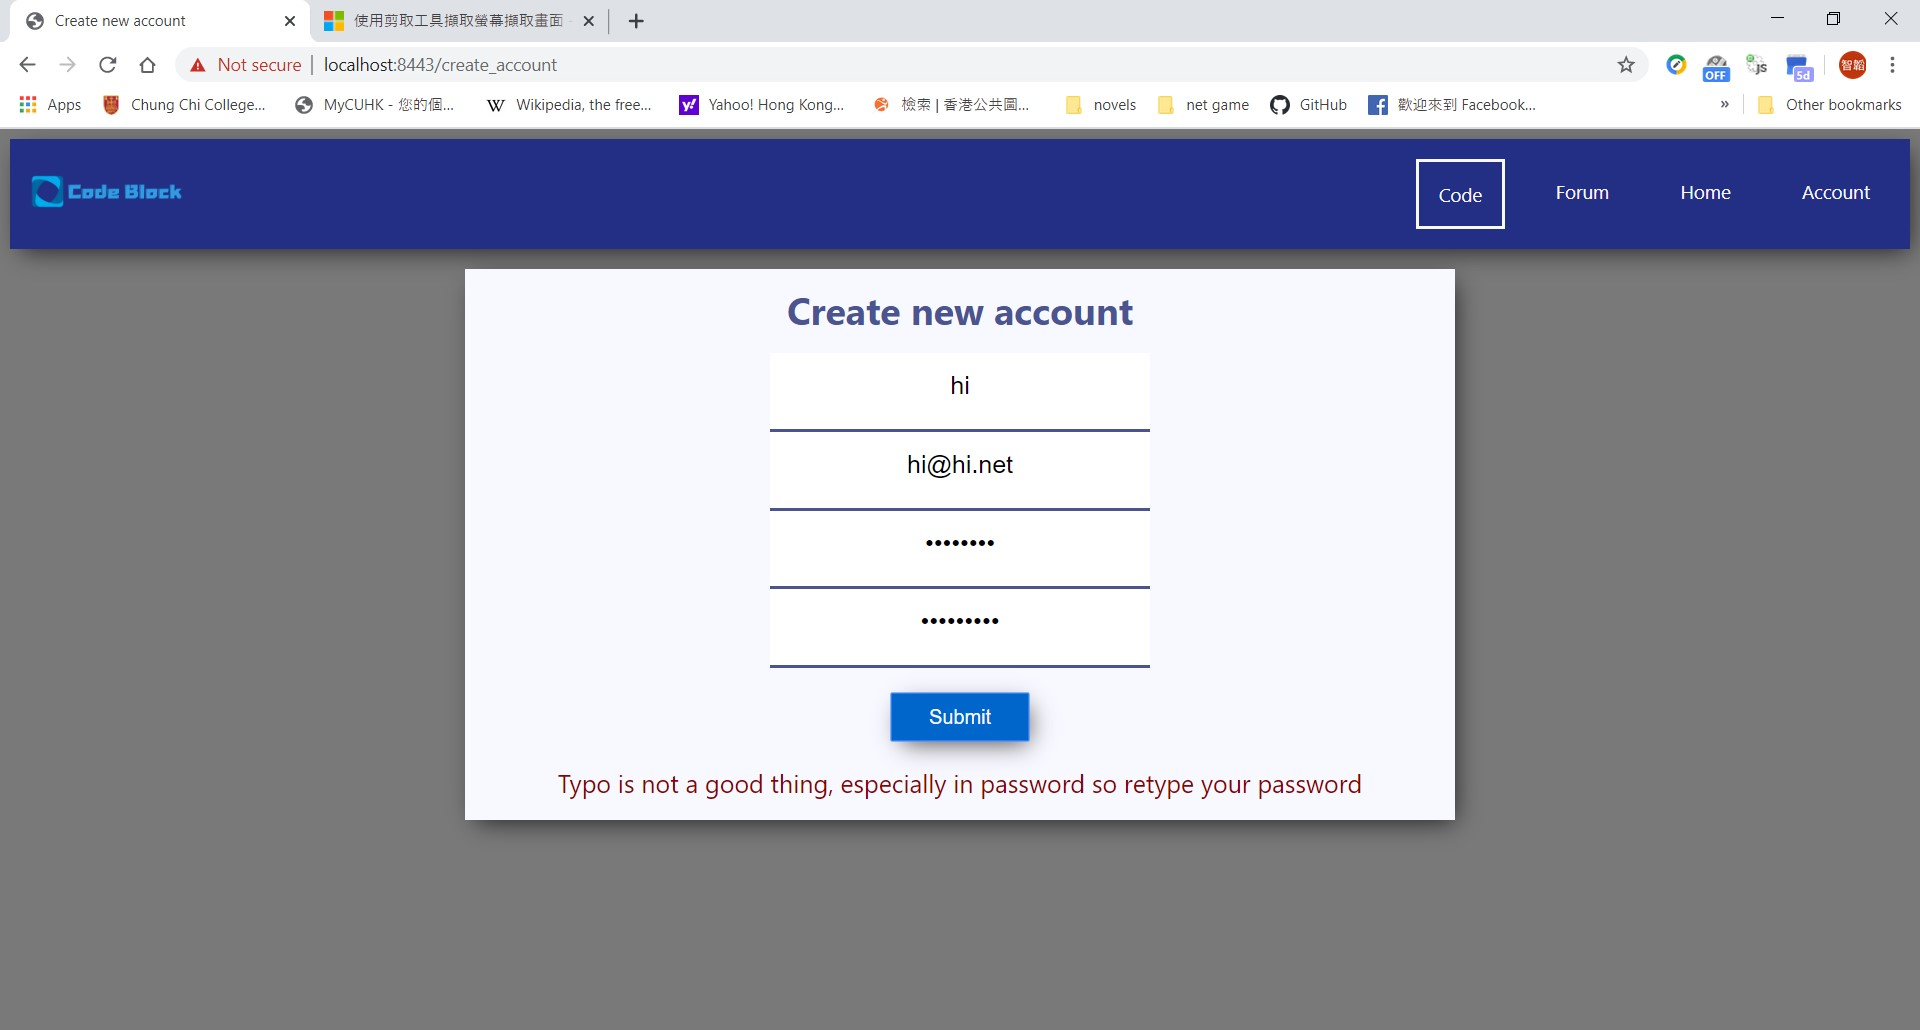
\includegraphics[scale=0.45]{Doc/Pics/case-5-1-9}

~

\subsubsection{User Account Authentication and User Data Retrieval}
Case 1: (pass)\\
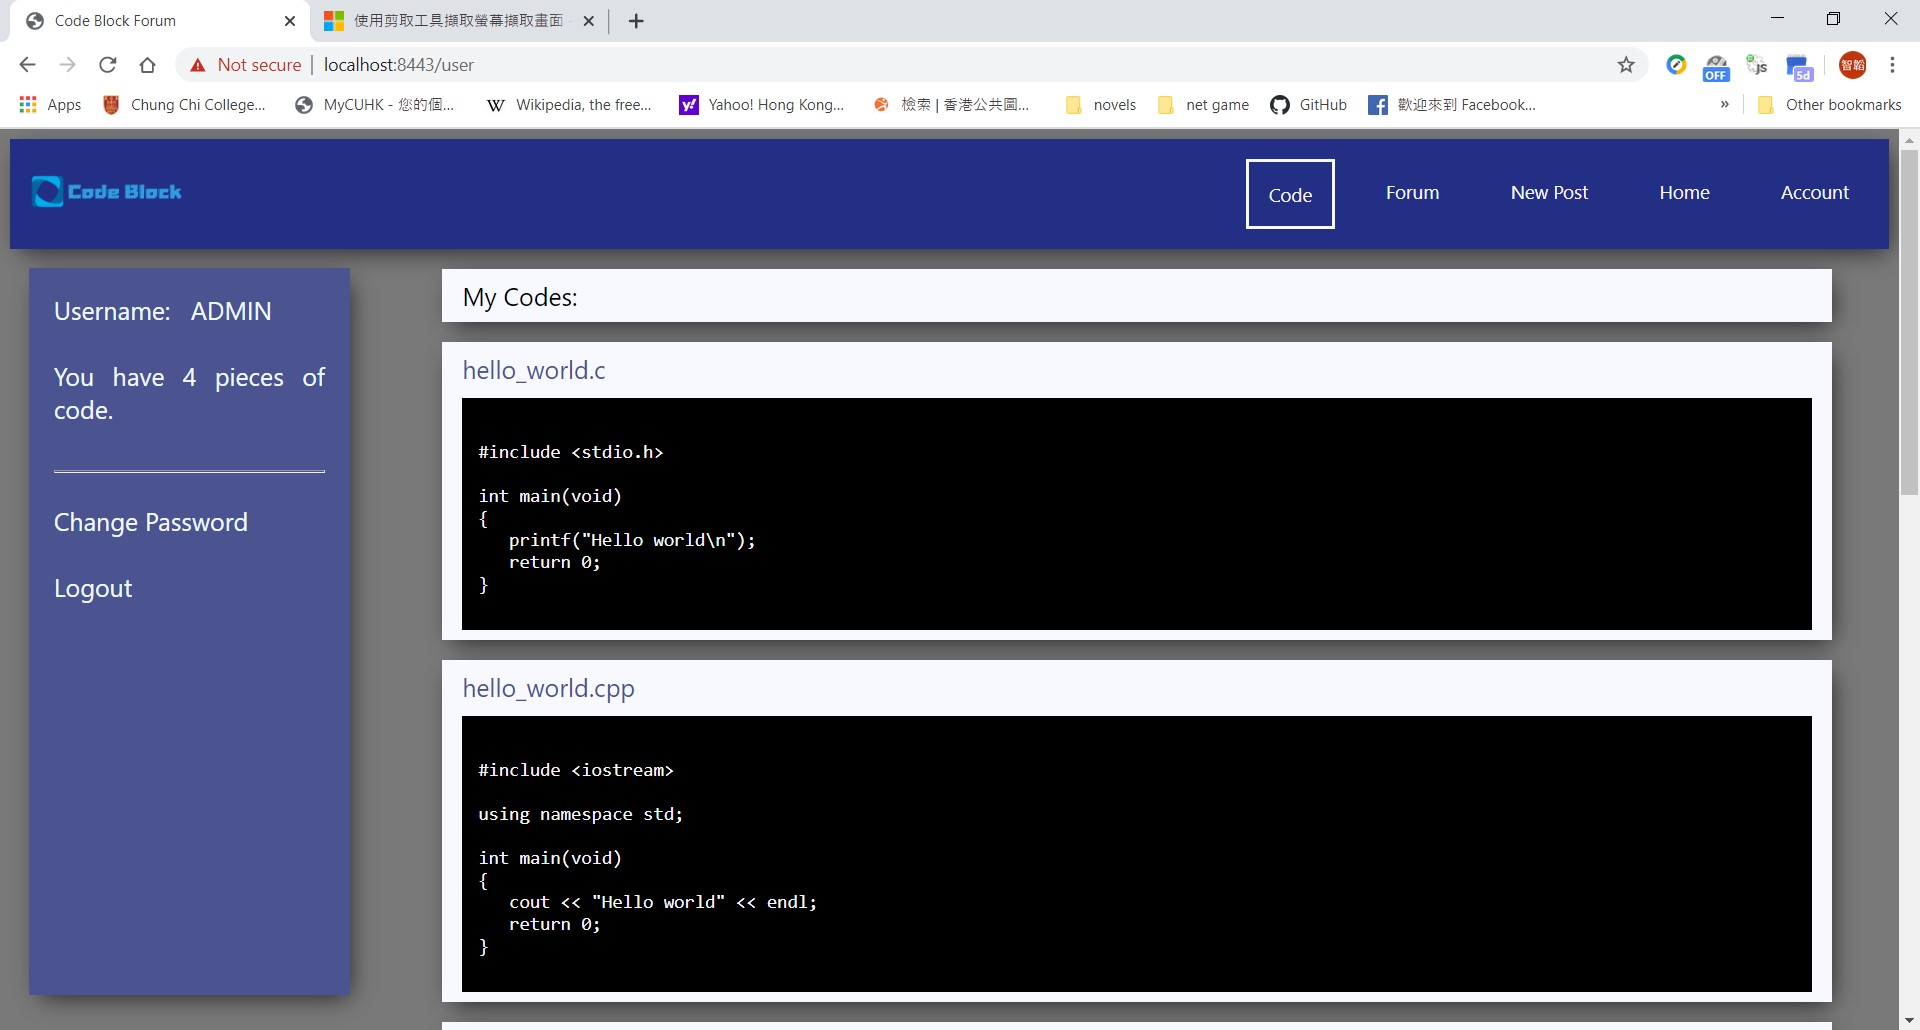
\includegraphics[scale=0.45]{Doc/Pics/case-5-2-1}

\paragraph{Logout}

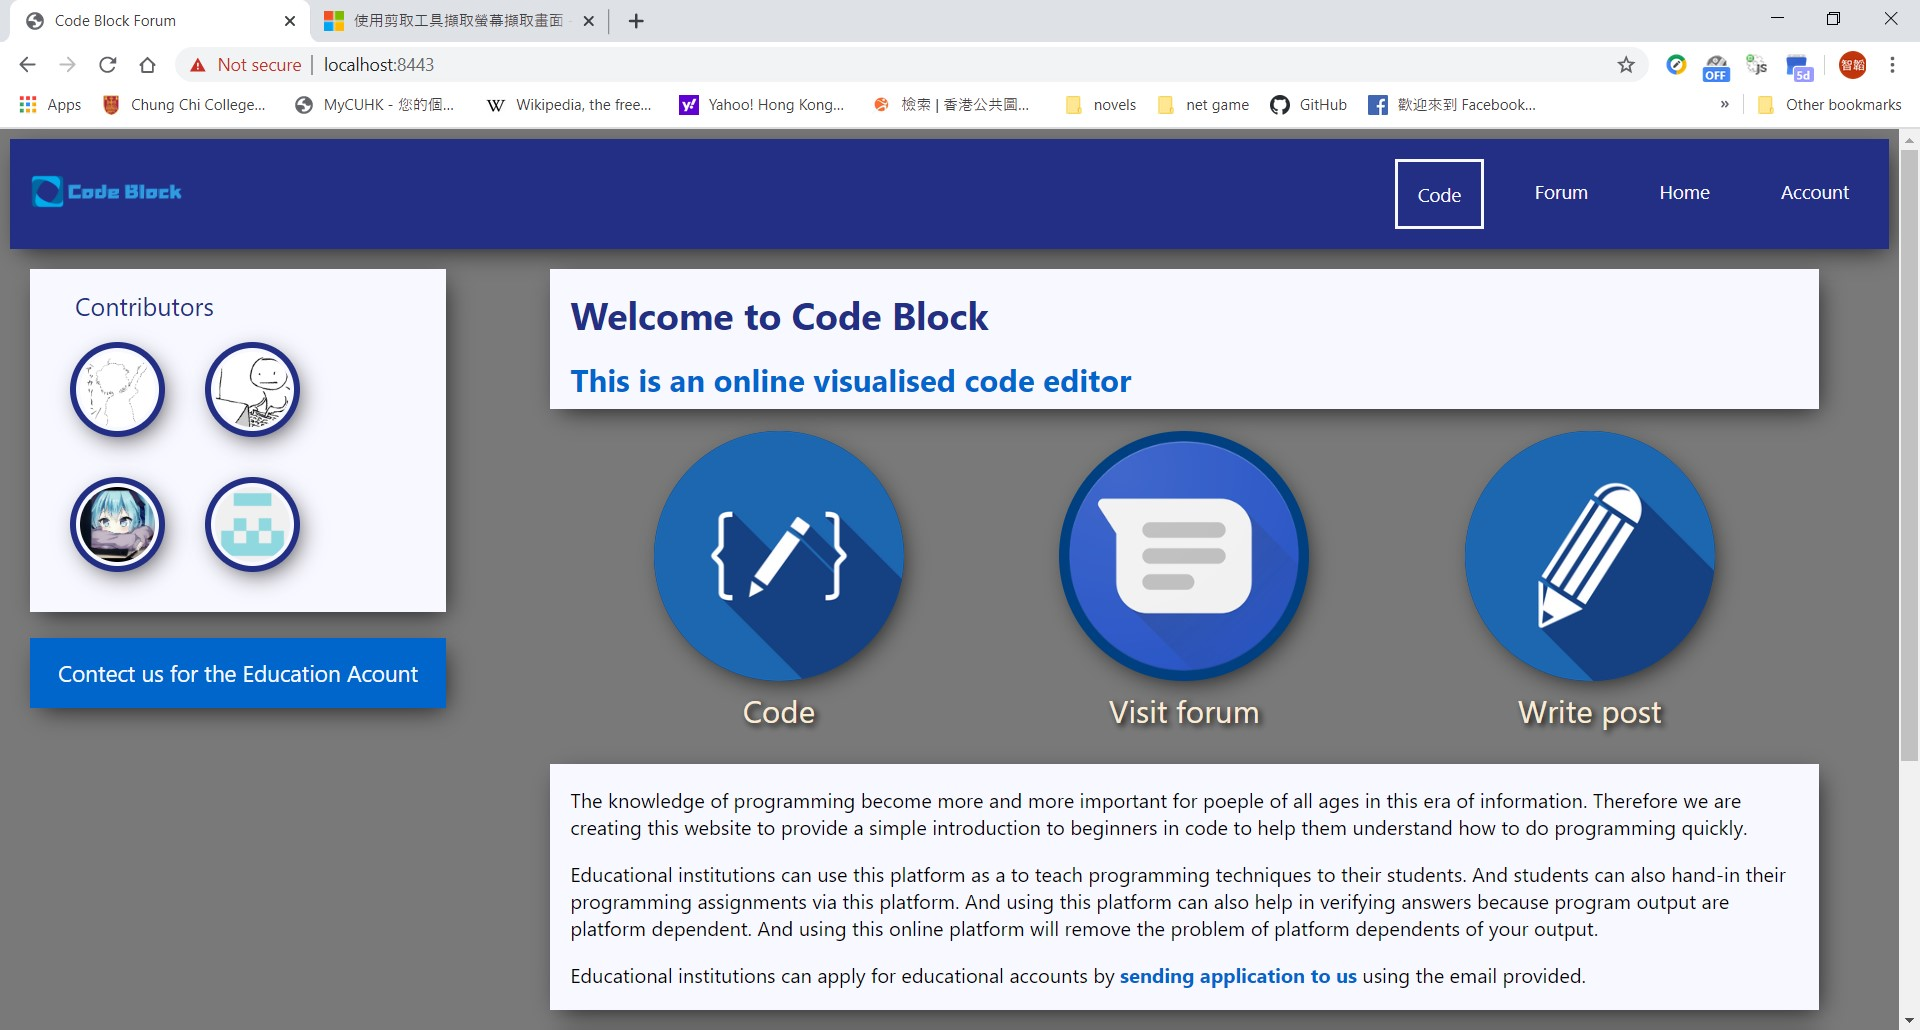
\includegraphics[scale=0.45]{Doc/Pics/logout}

~

Case 2: (pass)\\
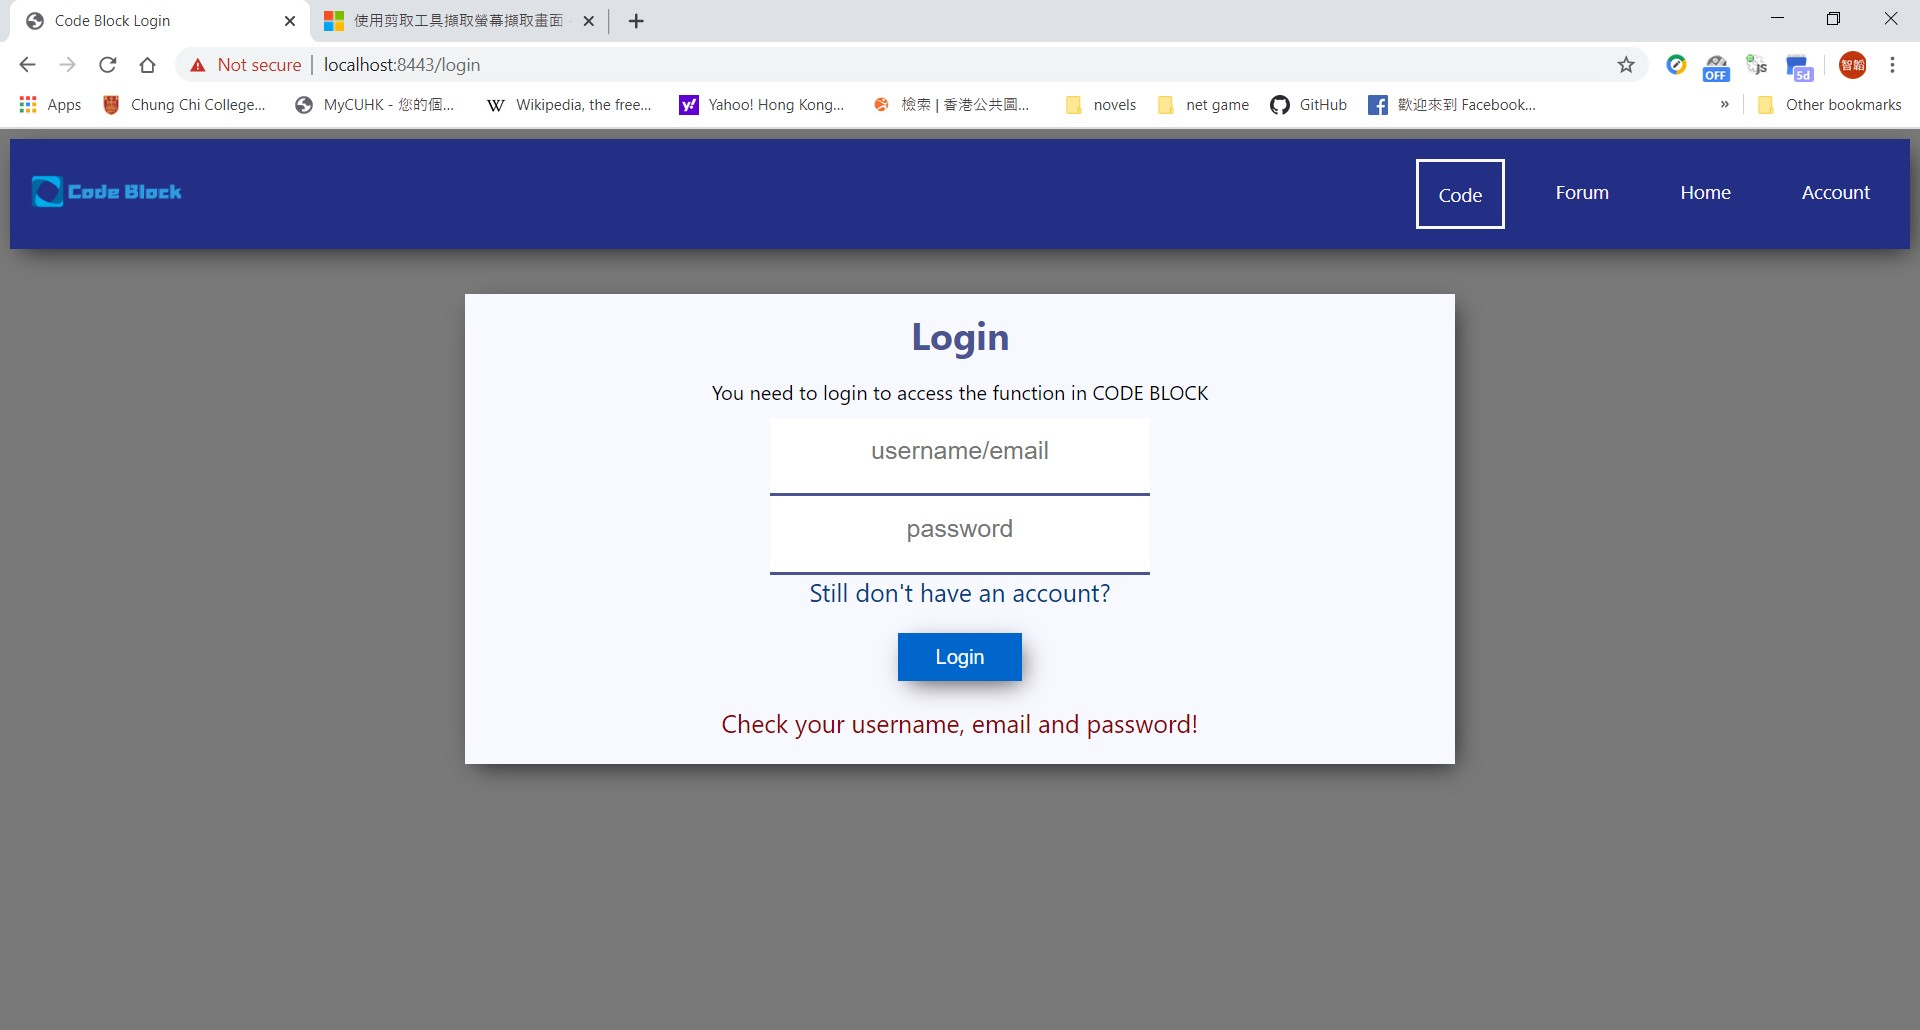
\includegraphics[scale=0.45]{Doc/Pics/case-5-2-2}

~

Case 3: (pass)\\
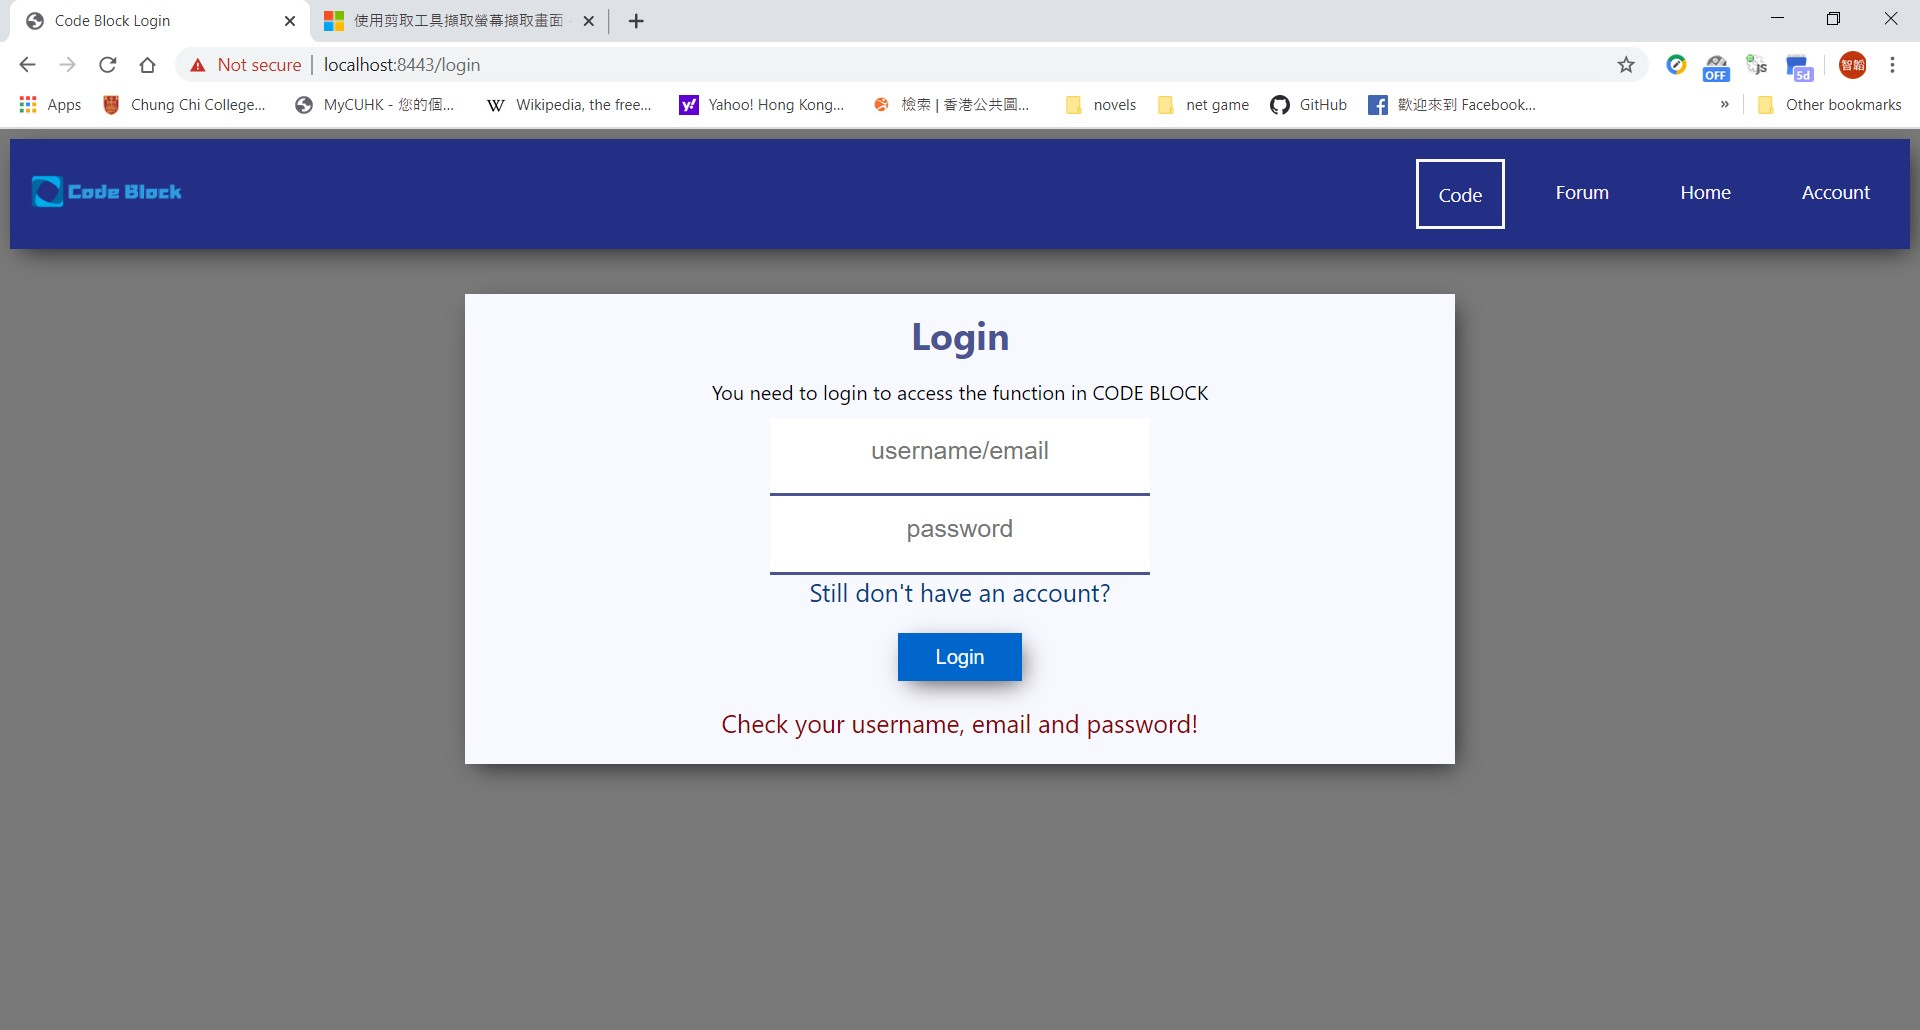
\includegraphics[scale=0.45]{Doc/Pics/case-5-2-3}

~

Case 4: (pass)\\
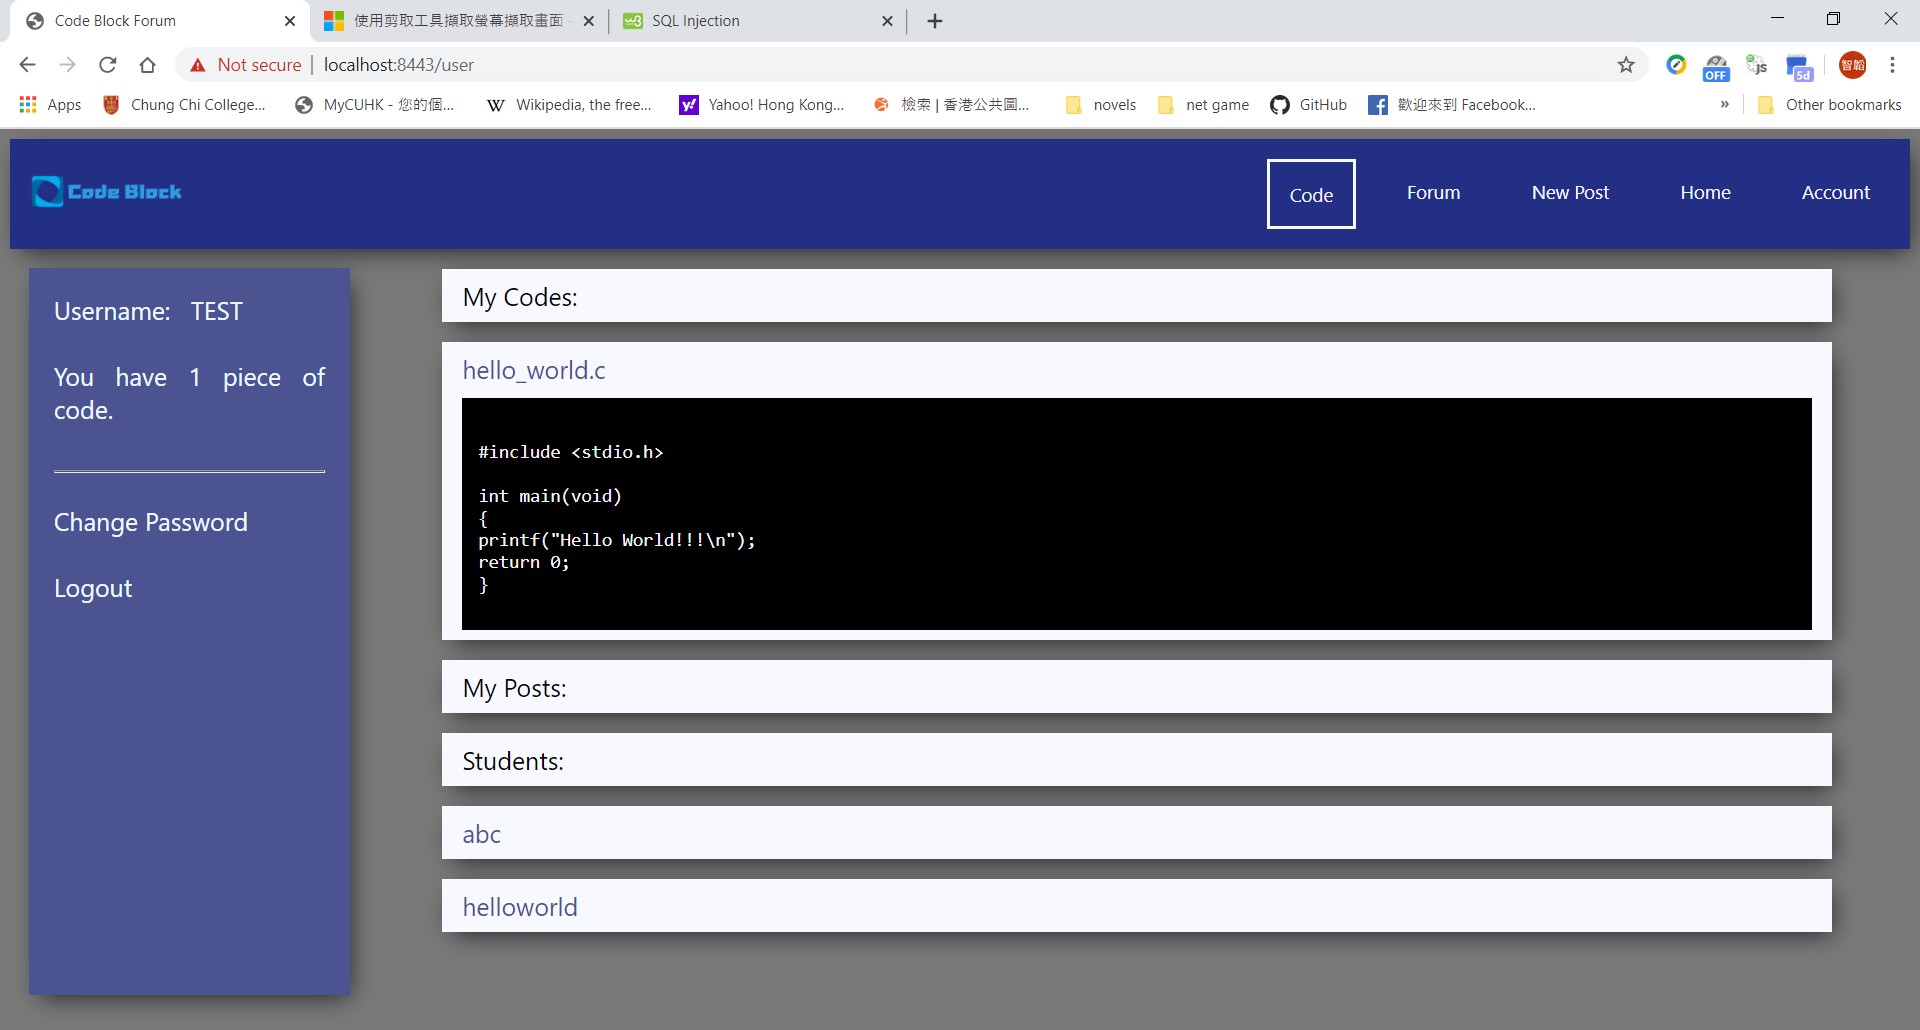
\includegraphics[scale=0.45]{Doc/Pics/case-5-2-4}

\paragraph{Logout}

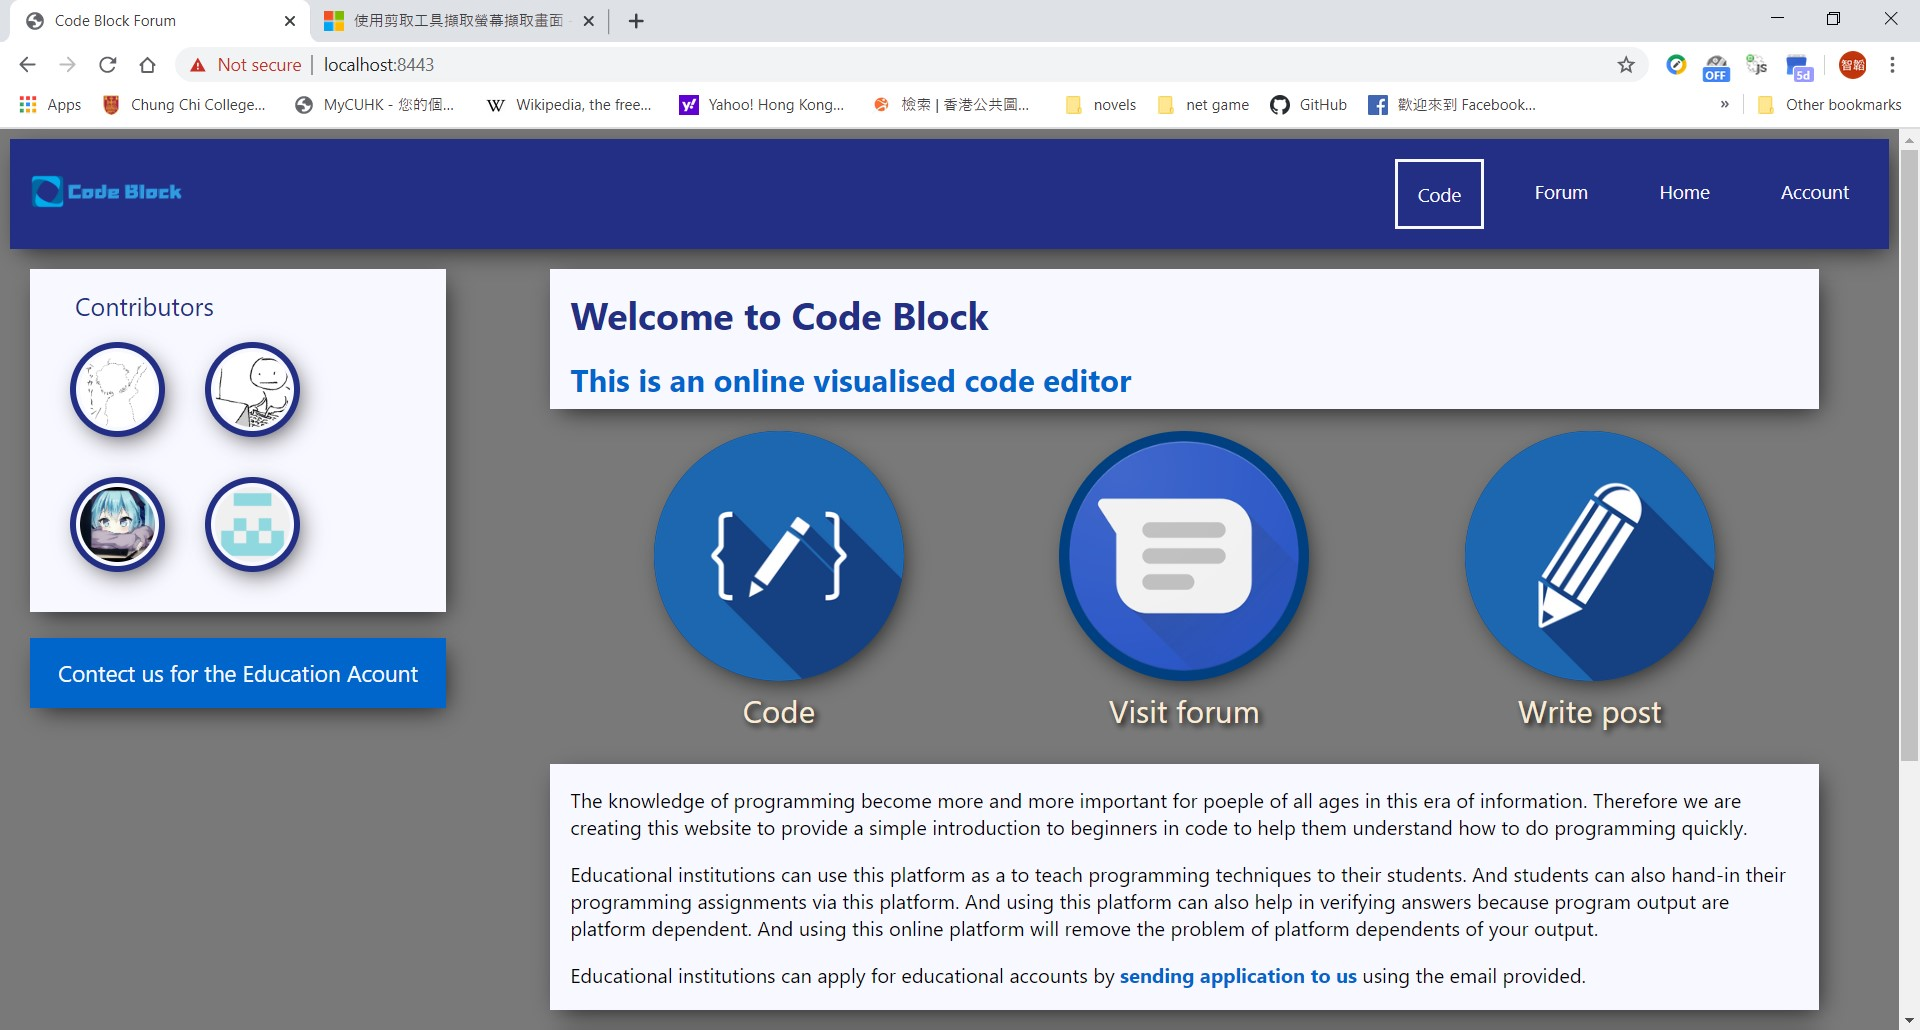
\includegraphics[scale=0.45]{Doc/Pics/logout}

~

Case 5: (pass)\\
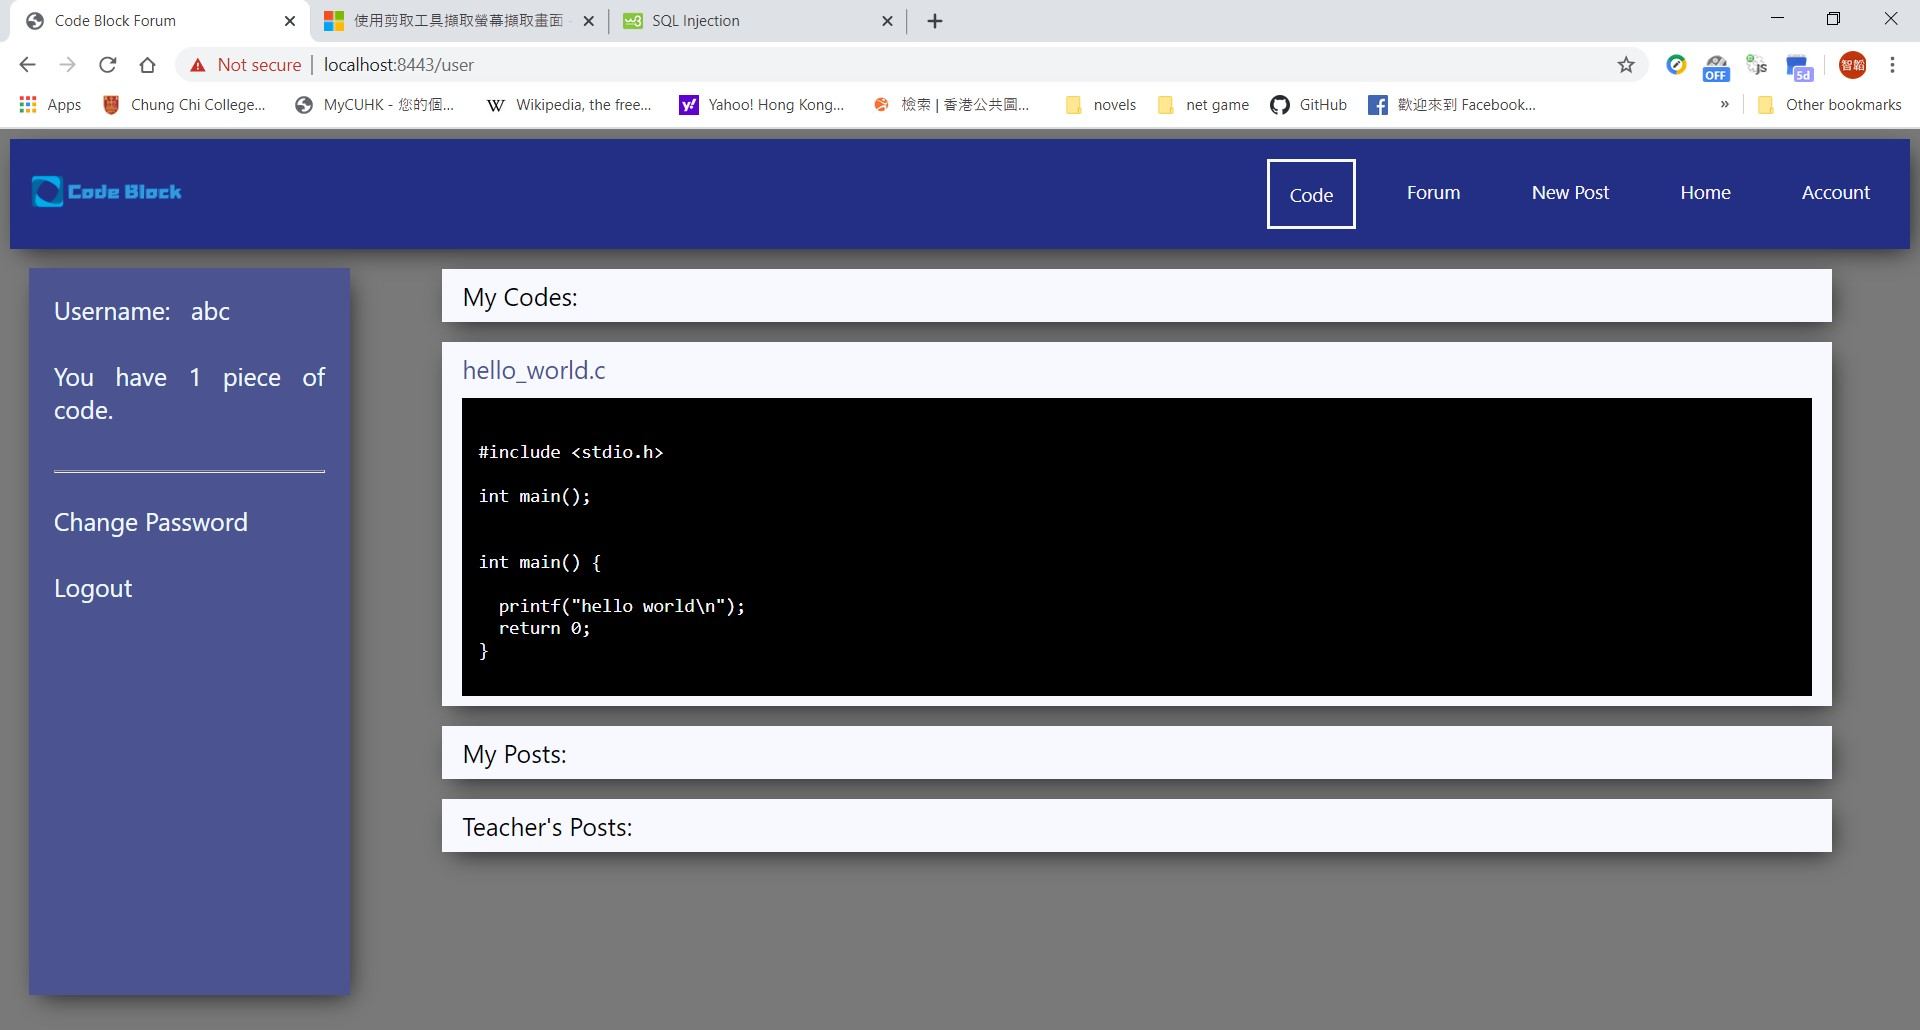
\includegraphics[scale=0.45]{Doc/Pics/case-5-2-5}

\paragraph{Logout}

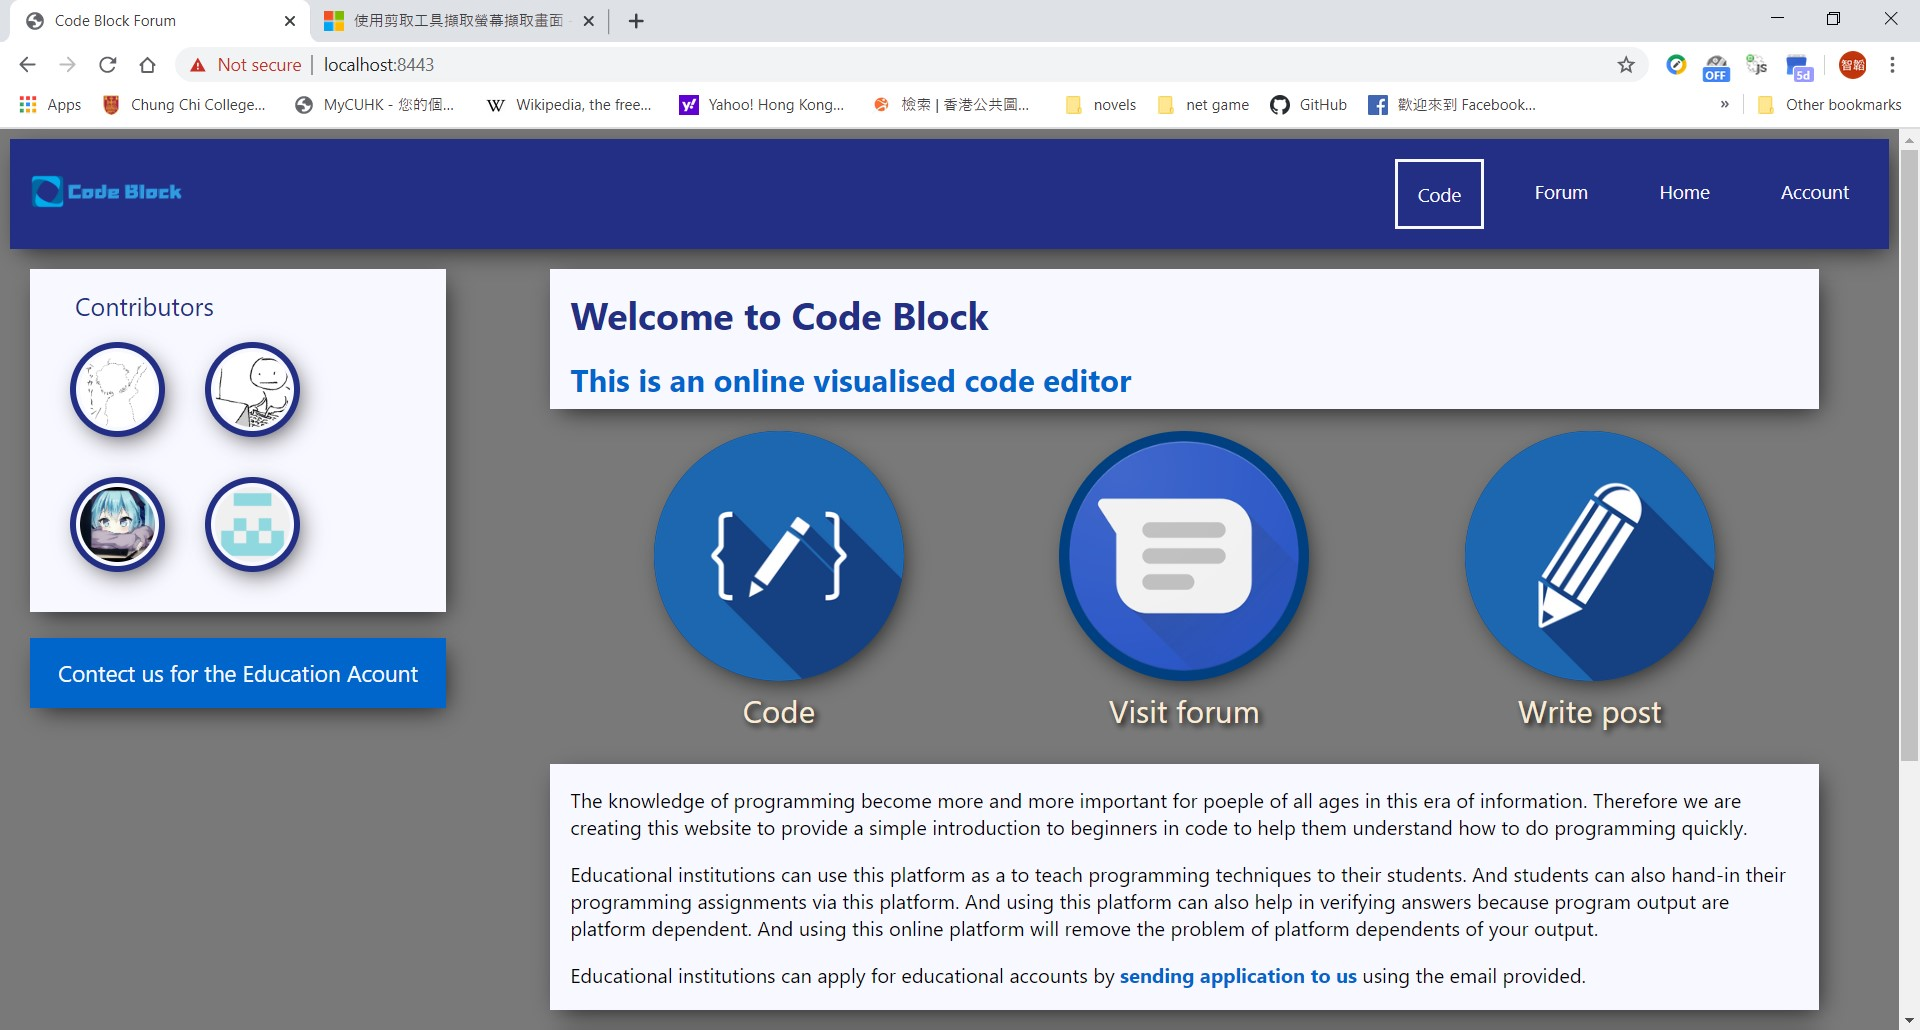
\includegraphics[scale=0.45]{Doc/Pics/logout}

~

Case 6: (pass)\\
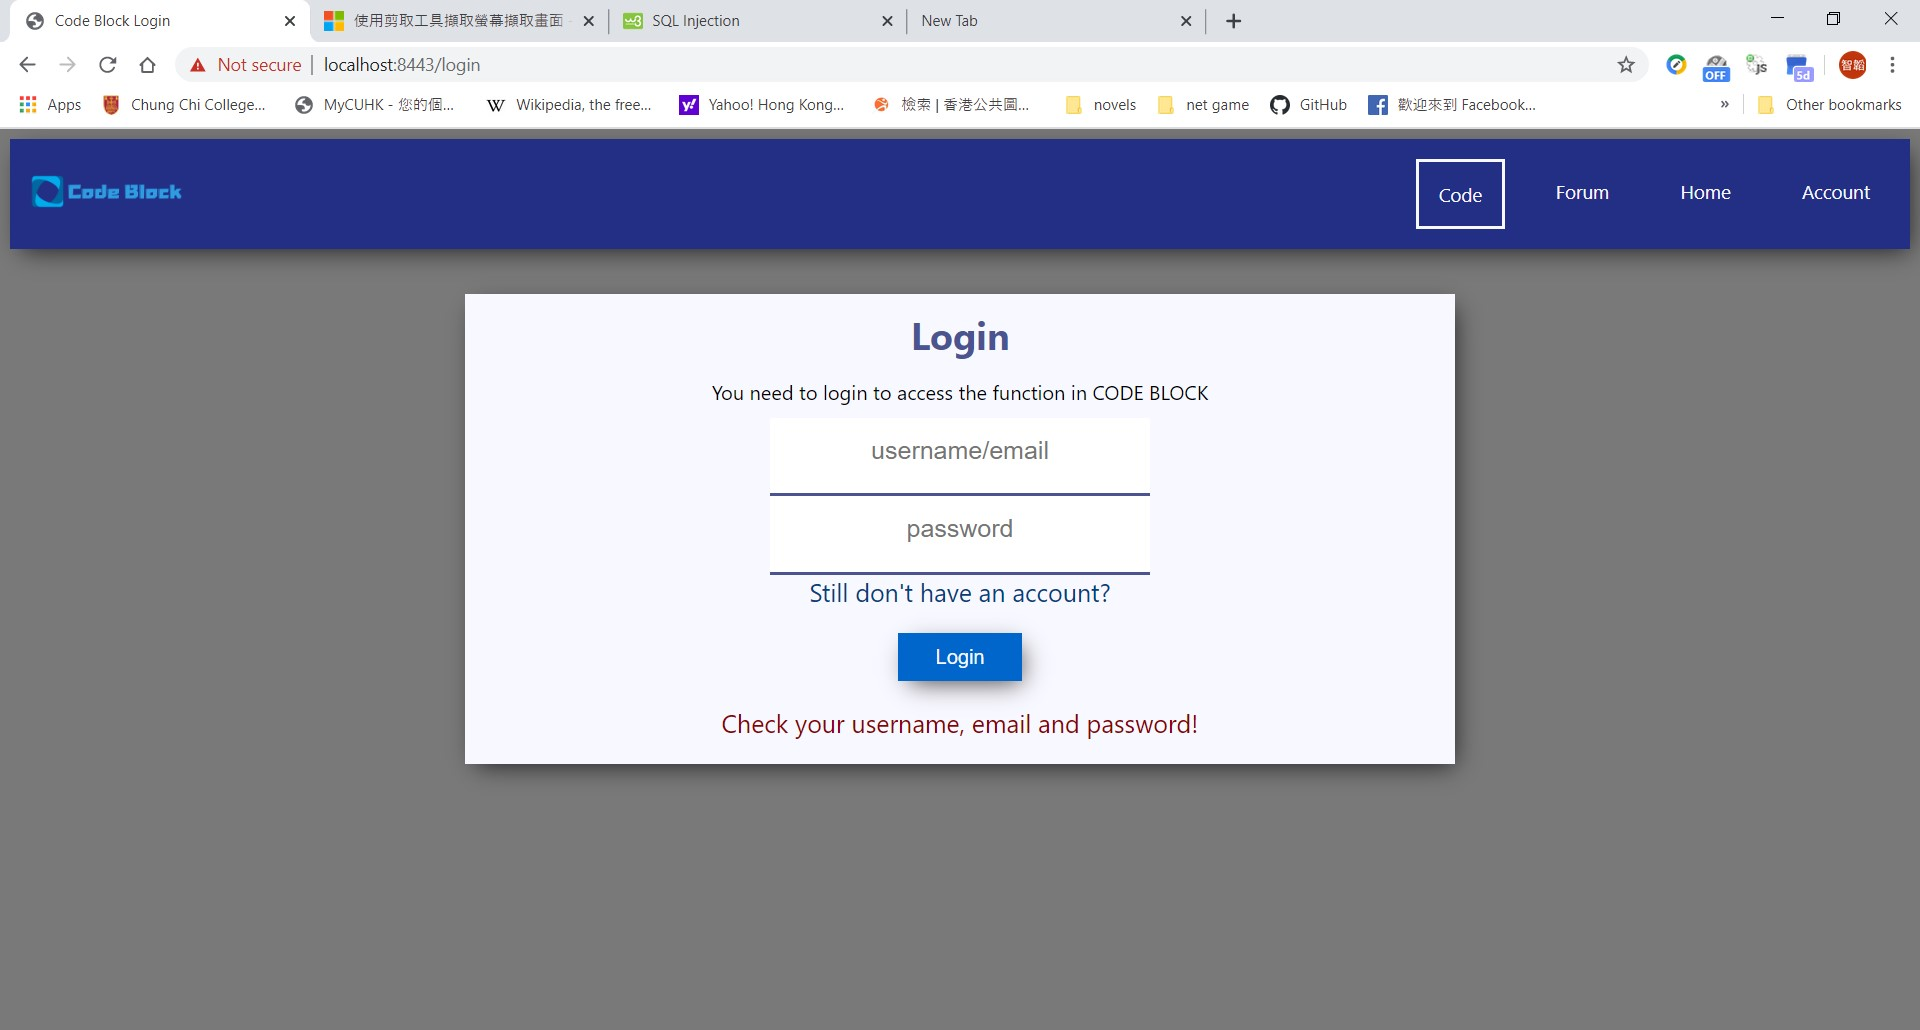
\includegraphics[scale=0.45]{Doc/Pics/case-5-2-6}

~

Case 7: (pass)\\
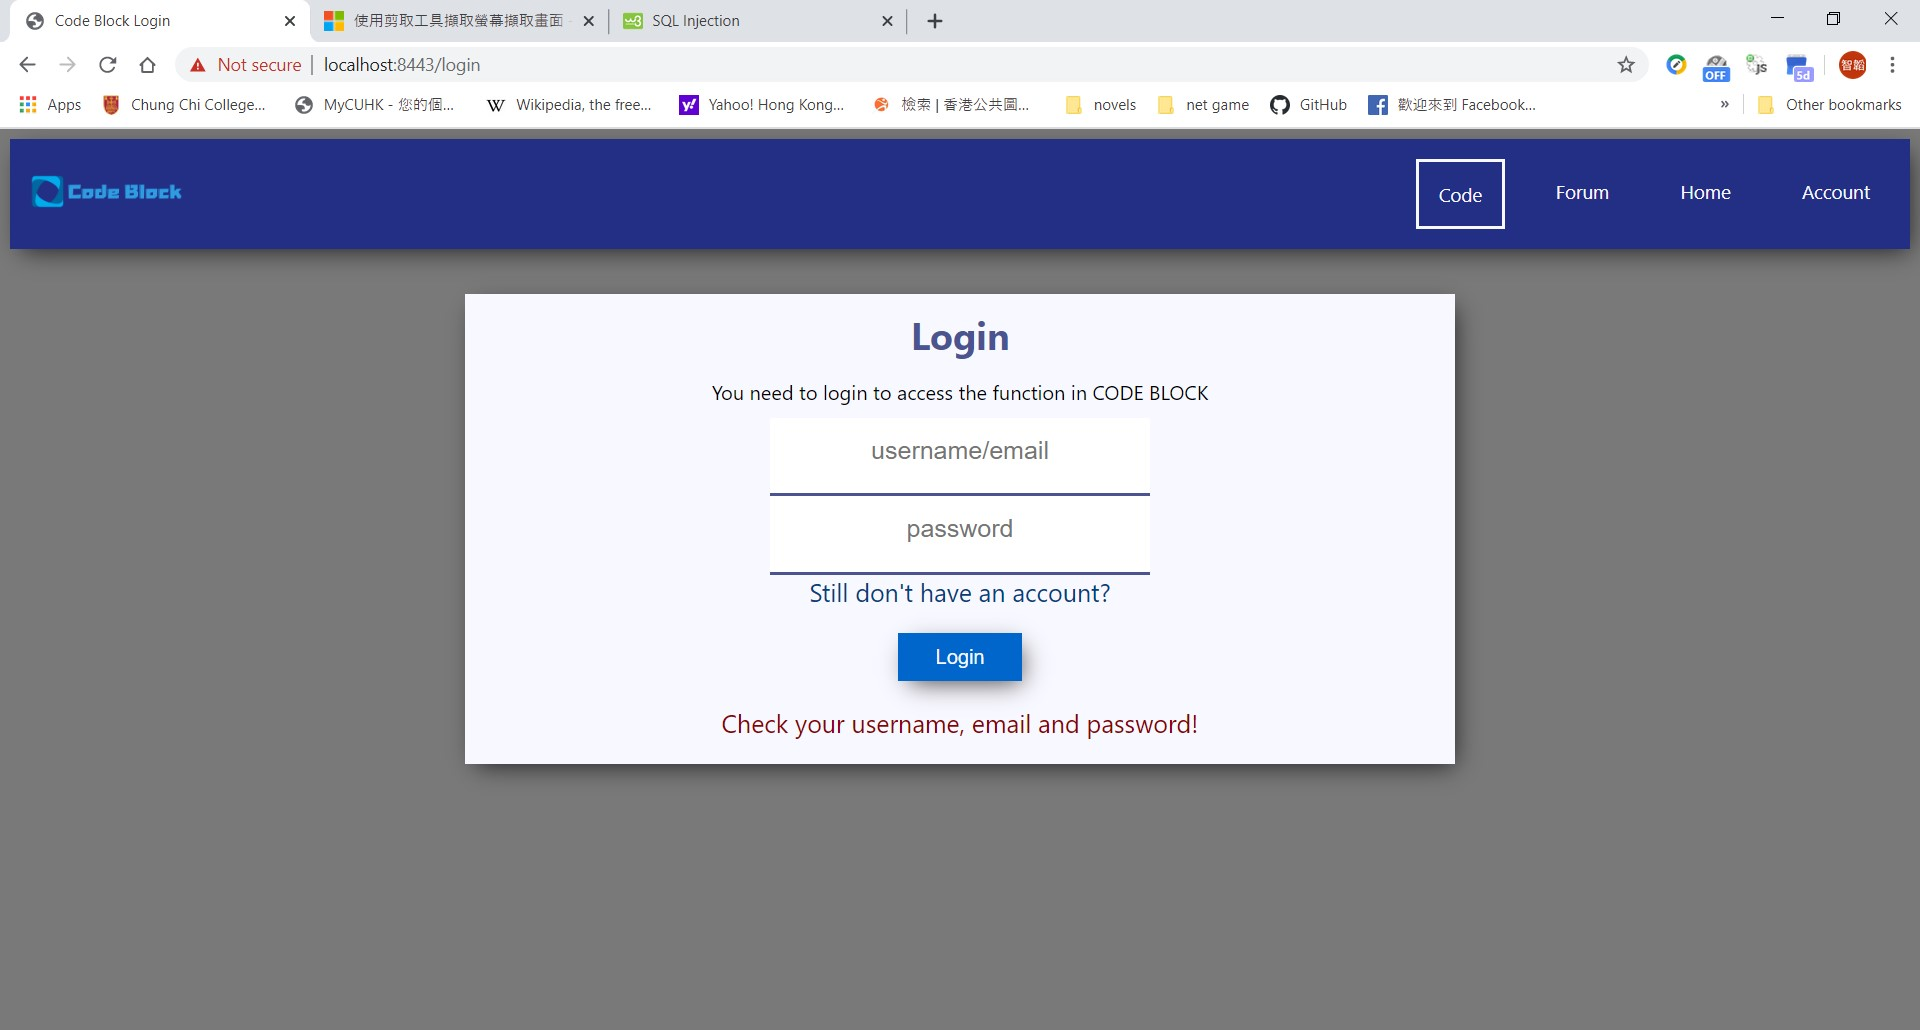
\includegraphics[scale=0.45]{Doc/Pics/case-5-2-7}

~

Case 8: (pass)\\
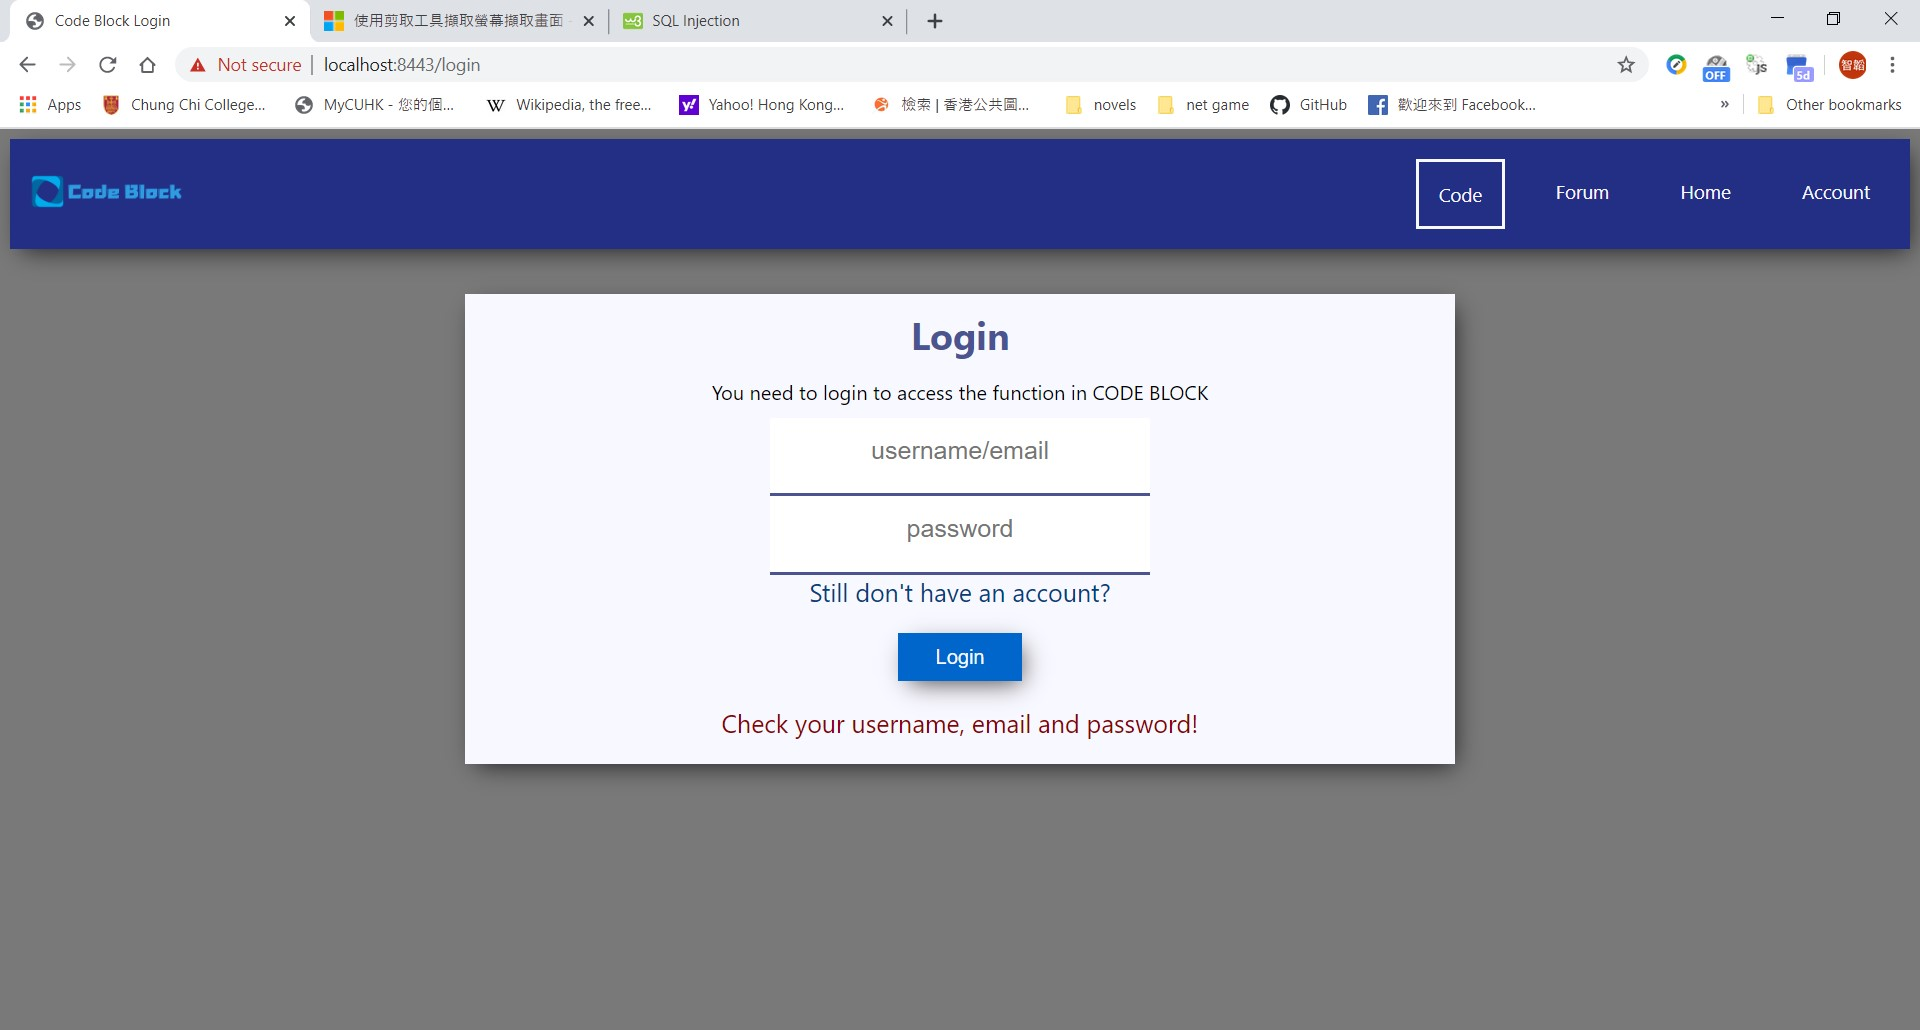
\includegraphics[scale=0.45]{Doc/Pics/case-5-2-8}

~

Case 9: (pass)\\
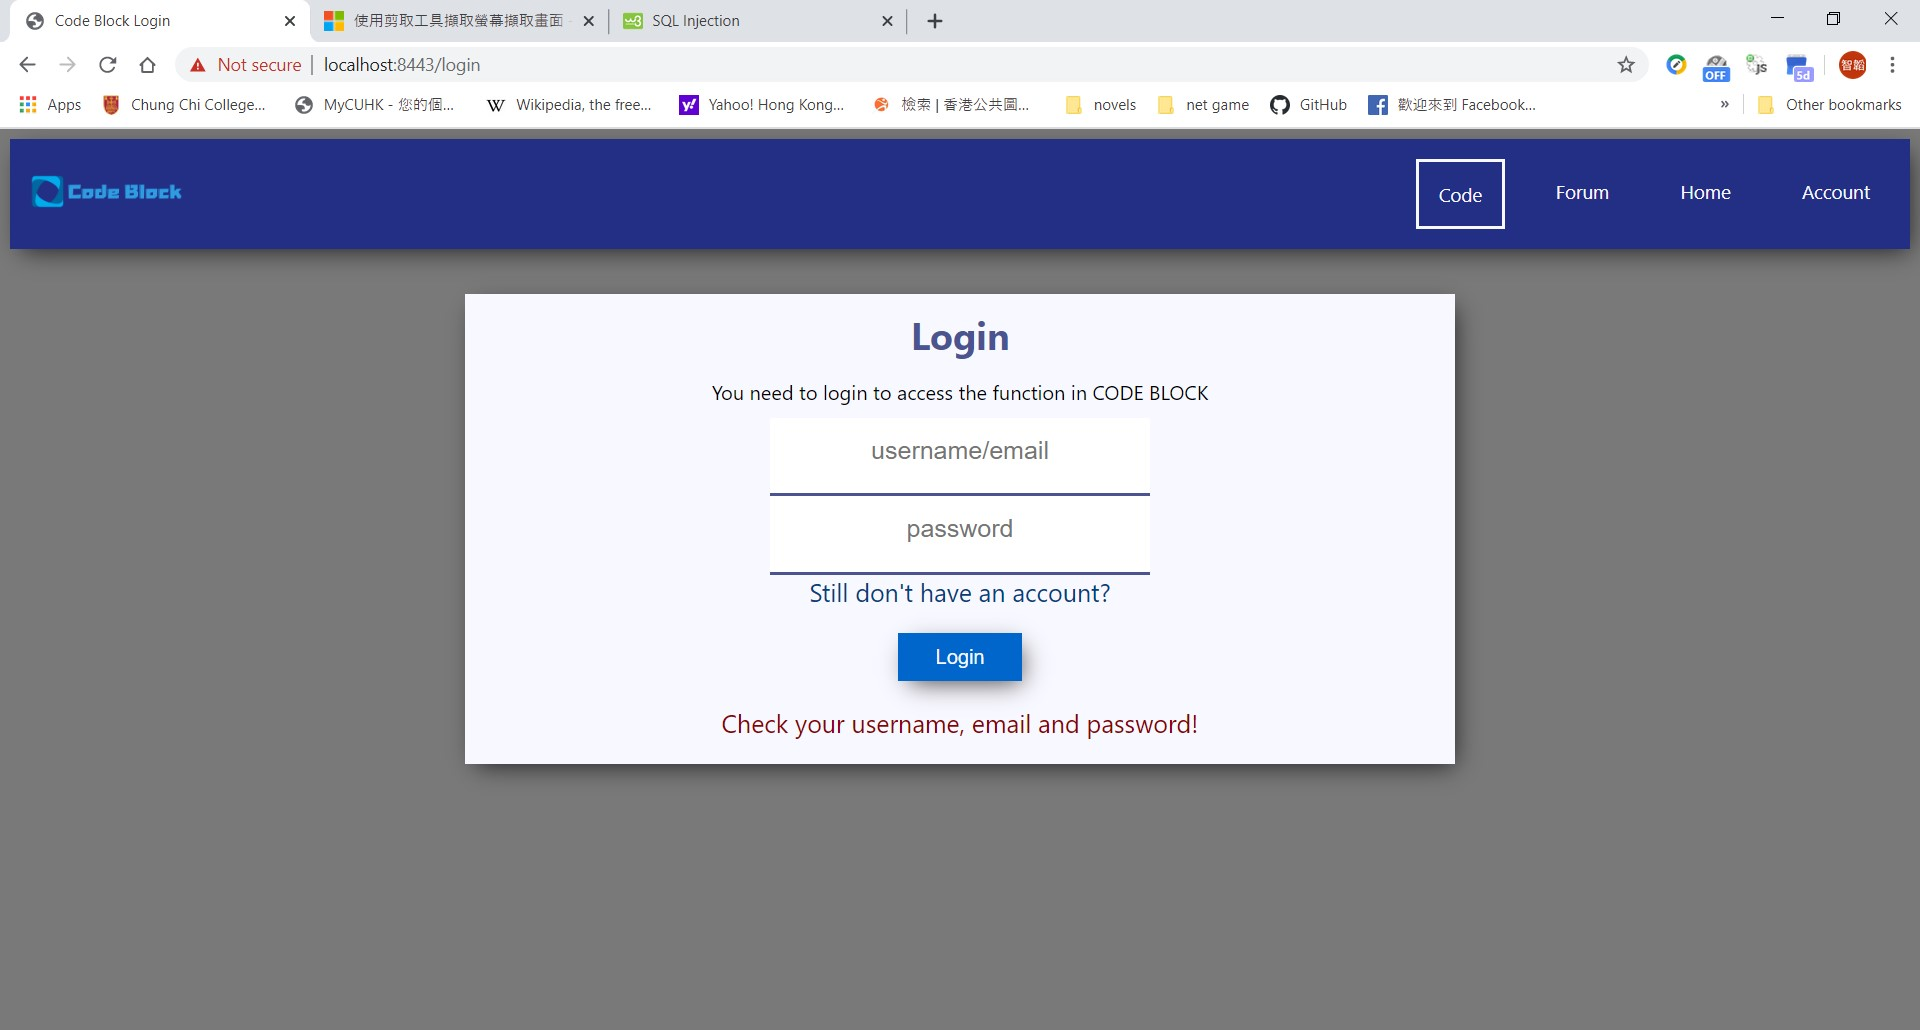
\includegraphics[scale=0.45]{Doc/Pics/case-5-2-9}

~

\section{Code Editing and Saving}

\section{Code Compilation and Running}

\section{Forum}
